\section{Briefverkehr mit Auftraggeberin}
\label{Briefverkehr mit Auftraggeberin}

\subsection*{Fragen}
\begin{enumerate} 
\item Wie soll der Besucher informiert werden, wenn er sich in einen verbotenen Bereich begibt?
\item Wie soll der Mitarbeiter informiert werden, wenn sich ein Besucher in einen verbotenen Bereich begibt?
\item Wie viele Audiodateien müssen in etwa auf dem Gerät gespeichert werden?
\item Wie lange sind die Audiodateien für die Kunstwerke im Durchschnitt in etwa?
\item Wir benötigen einen genauen Plan des Gehäuses des Dojos. Insbesondere die Position und Dimensionen der Einbuchtung für die Schalter ist sehr wichtig.
\item Bei der Vorstelung hiess es, dass das Gehäuse in einem 3D-Drucker hergestellt wurde. Können sie uns das dazugehörige (stl)-File zukommen lassen?
\item Ist es vorgesehen, dass das Gehäuse geöffnet werden kann? (Auswechseln des Akkus)
\item Ist eine Öffnung für den Knochenschallgeber vorgesehen oder befindet sich dieser innerhalb des Gehäuses?
\item Angenommen der Besucher steht vor einem Ausstellungsstück und hört sich den dazugehörigen Audioclip an. Er läuft nun (während die Wiedergabe weiterläuft) zu einem neuen Objekt. Soll in diesem Falll ein Feedback(Vibration, LED) an den Besucher gesendet werden, dass er sich nun bei einem neuen Objekt befindet? Oder soll die Wiedergabe gestoppt werden? Soll sie weiterlaufen?
\item Angenommen der Besucher steht vor einem Ausstellungsstück und hört sich den dazugehörigen Audioclip an. Er pausiert nun die Widergabe und läuft anschliessend zu einem neuen Objekt. Daraufhin erhält er ein Feedback vom Dojo, welches ihm sagt, dass er nun bei einem neuen Objekt ist. Wenn der Besucher jetzt den Play-Button drückt, soll dann die pausierte Audiodatei des vorherigen Objektes weiter abgespielt werden oder soll die Audiodatei des neuen Objektes abgespielt werden?
\item Die Idee laut Spezifikationen des Dojos besteht darin, dass am Ende ein PDF o.Ä erstellt wird. Die Daten dazu befinden sich irgendwo in der Infrastruktur des Museums. Auf diese Daten haben wir ja kein Zugriff, d.h. das linken der gesammelten Informationen auf dem Dojo mit der Datenbank ist dann Sacher der internen IT des Museums. Wir können also nur die Schnittstelle dazu liefern. Die Frage ist nun, in welcher Form wir die Information eines gelikten Ausstellungsstückes liefern sollen?
\end{enumerate}

\newpage
\subsection*{Antworten}
\begin{enumerate}
\item Ich denke du sprichst hier das Tracking des Besuchers in den verschiedenen Umgebungen/Zonen an. Das Eintreten in einen gesonderten Bereich (Sammlung, Dauerausstellung etc) müsste durch eine RFID Schranke geregelt werden. Im konsequentesten Szenario ist dies ein Drehkreuz welches mit dem programmierten Dojo/Ticketbadge aktiviert wird. Denkbar ist aber auch ein Personalmitarbeiter mit einem Scan-Gerät, welcher die Besucher eintreten lässt. Insofern gibt es keinen verbotenen Bereich. Es ist denkbar, dass besagter Durchgang gerade nicht von einem Personalmitarbeiter oder Drehkreuz/Schranke bedient wird. In diesem Fall könnte das System lediglich eine Meldung an das Museum/Monitorig auslösen, dass sich jemand in einem Bereich befindet, für welchen er keine ‚Zutrittsrechte‘ hat. Grundsätzlich sollte das Dojo nicht ‚Alarm‘ schlagen. 
Für Gegenvorschläge bin ich offen.

\item Der Mitarbeiter bezieht diese Information von einem Endgerät der CMS Software. Sei dies ein Smartphone, Smartwatch oder anderer Computer. Die Frage des ‚Wie‘ sollte variabel bleiben. Das System benachrichtigt den Mitarbeiter in Form einer neuen Meldung über das Dojo-Endgerät, welches sich in einem anderen (suboptimalen) Bereich befindet und dessen Standort.

\item Auf dem Gerät sollte es Platz haben für 2-4 GB Daten. Ich beantworte die Frage so, weil die Menge an Audiodateien variabel ist.

\item Dies kann unterschiedlich ausfallen. Eine oberflächliche Recherche meinerseits hat ergeben, das Beiträge zu Einzelstücken zwischen 01:00 – 02:30 lang sind.
Im Anhang habe ich zwei Sprachsample aus dem Metropolitan Museum of Art angehängt. Beide sind nicht länger als 3:00 Minuten.

\item Ich habe einen Plan der verschiedenen Ansichten erstellt. Er ist im Anhang.

\item Zu diesem Thema werde ich mich noch mit Herrn Gysin und Meier austauschen. Derzeit habe ich eine Gehäusezeichnung und zwei separate Knöpfe als stl.

\item Eine Öffnung ist vorgesehen. Die ganze Rückseite sollte herausschiebbar sein. Anbei eine Grafik.

\item Der Signalgeber befindet sich im Gehäuse, jedoch sollte die Membrane einen festen Kontakt zu der Auflagefläche (geschwungene Fläche) des Dojo gewährleisten. So wird das Vibrations-Signal zuerst an die Auflagefläche, dann weiter an den Knochen weitergegeben.

\item Das Dojo bleibt empfangsbereit. Bewegt sich also der Besucher weiter in der Ausstellung, reagiert auch das Smartdevice auf diese Bewegung. Natürlich wird er auch in den neuen Räumen getrackt, auch wenn er noch eine Audiodatei aus einem vorangehenden Raum hört.

\item Ich denke auch hier sollte ein standortbezogenes Feedback den Priorität haben. Der Besucher steht nun vor einem ‚aktuellen‘ Objekt und erhält die Möglichkeit sich dieses anzuhören.
Ich bin in diesem Punkt offen für UX-Gegenargumente.

\item Ich bin mir nicht sicher, ob ich die Frage richtig verstanden habe. Solche Datenbanken gehören meist zum festen Bestandteil der Kunstvermittlung solcher Institutionen und sind open source. Siehe anbei das Archiv des Kunstmuseum Basel . Dort gibt es unzählige Beispiele von Auszügen aus Werkbeschrieben. Um die Idee dieses PDF-Souvenirs zu verdeutlichen, habe ich anbei ein File angehängt. Es ist auch als gedruckte Broschüre denkbar. 
Ich bin damit einverstanden, dass das Museum einen IT-Mindestaufwand betreiben muss, um das Dojo System optimal in sein digitales Dasein zu integrieren.



\end{enumerate}

\newpage
  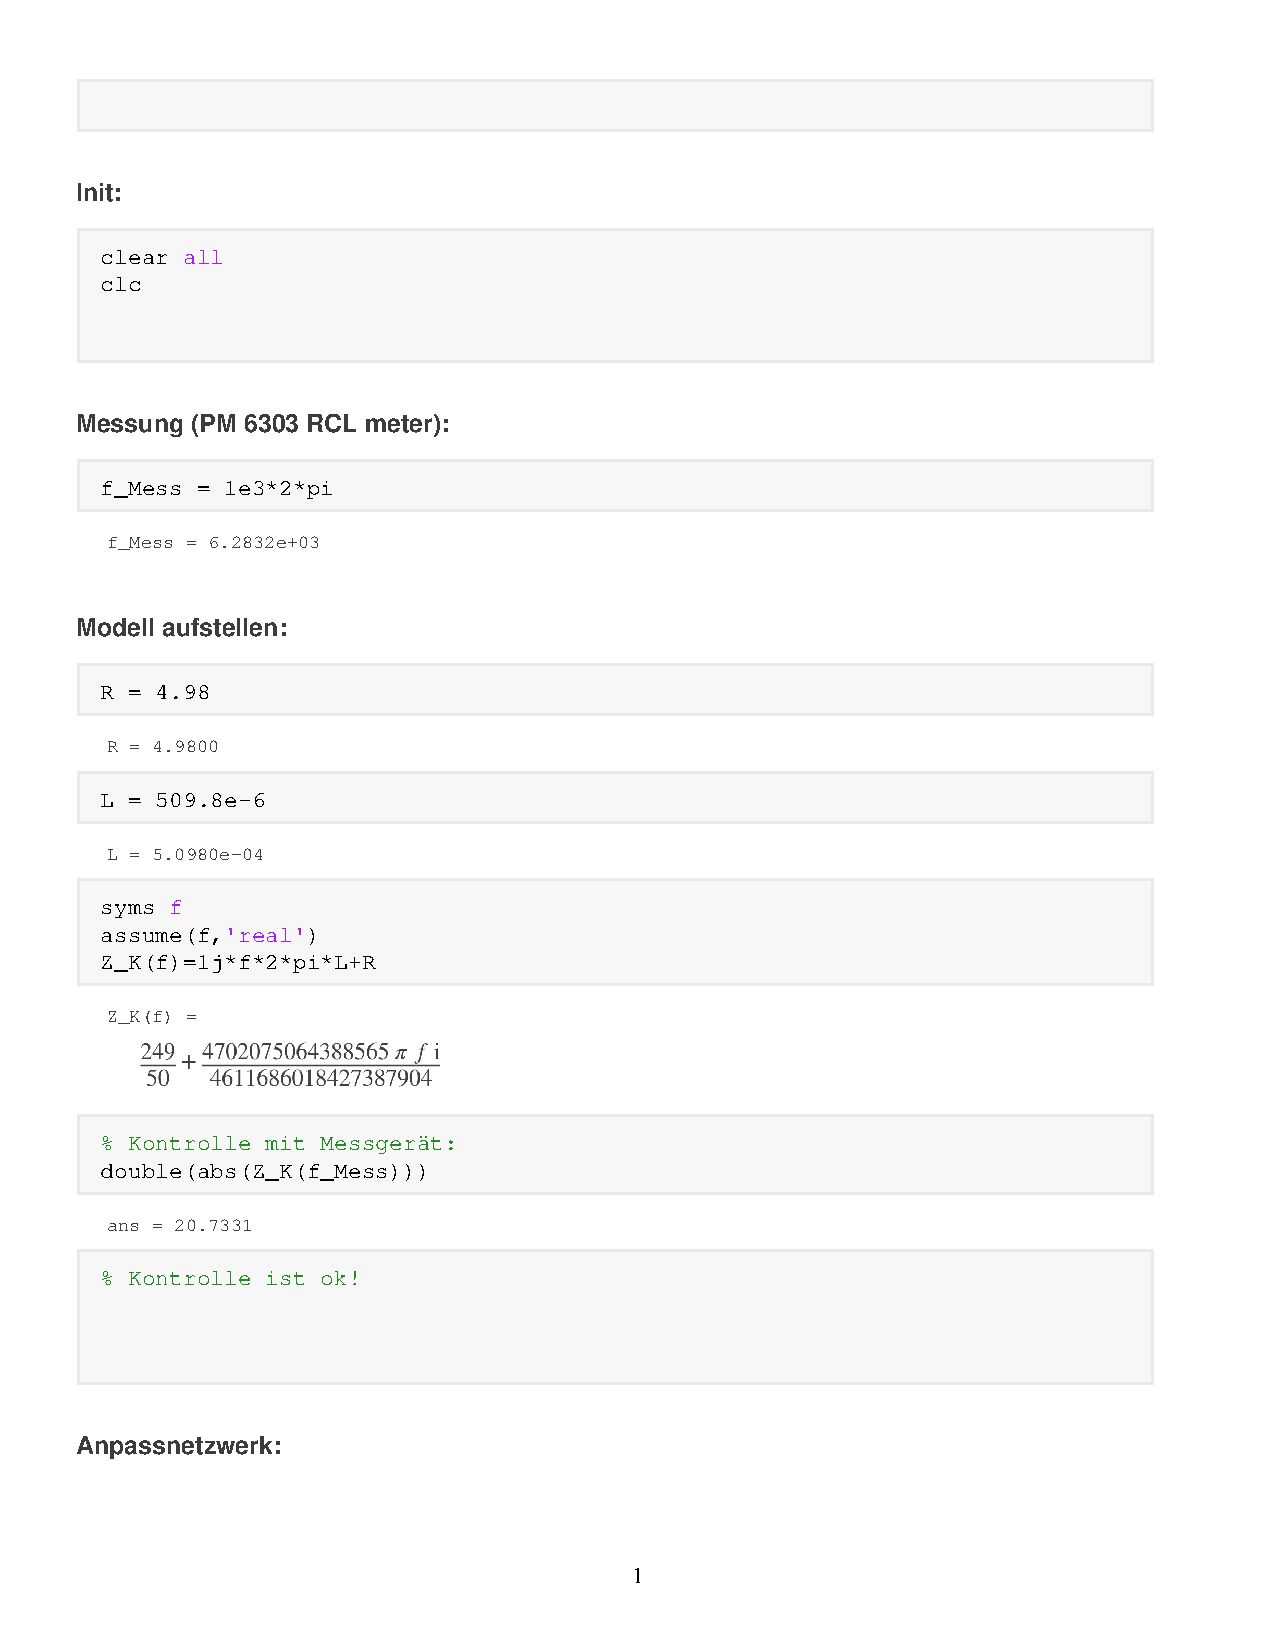
\includepdf[scale=0.8,pages=1,pagecommand=\section{Matlab Dokument zur Impedanzanpassung Knochenschallgeber}\label{fig:matlab_anhang}]{graphics/Knochenschallgeber_Matlab}
  \includepdf[scale=0.8,pages=2]{graphics/Knochenschallgeber_Matlab}
  \includepdf[scale=0.8,pages=3]{graphics/Knochenschallgeber_Matlab}

\newpage

\section{Aufbau des Dojos}

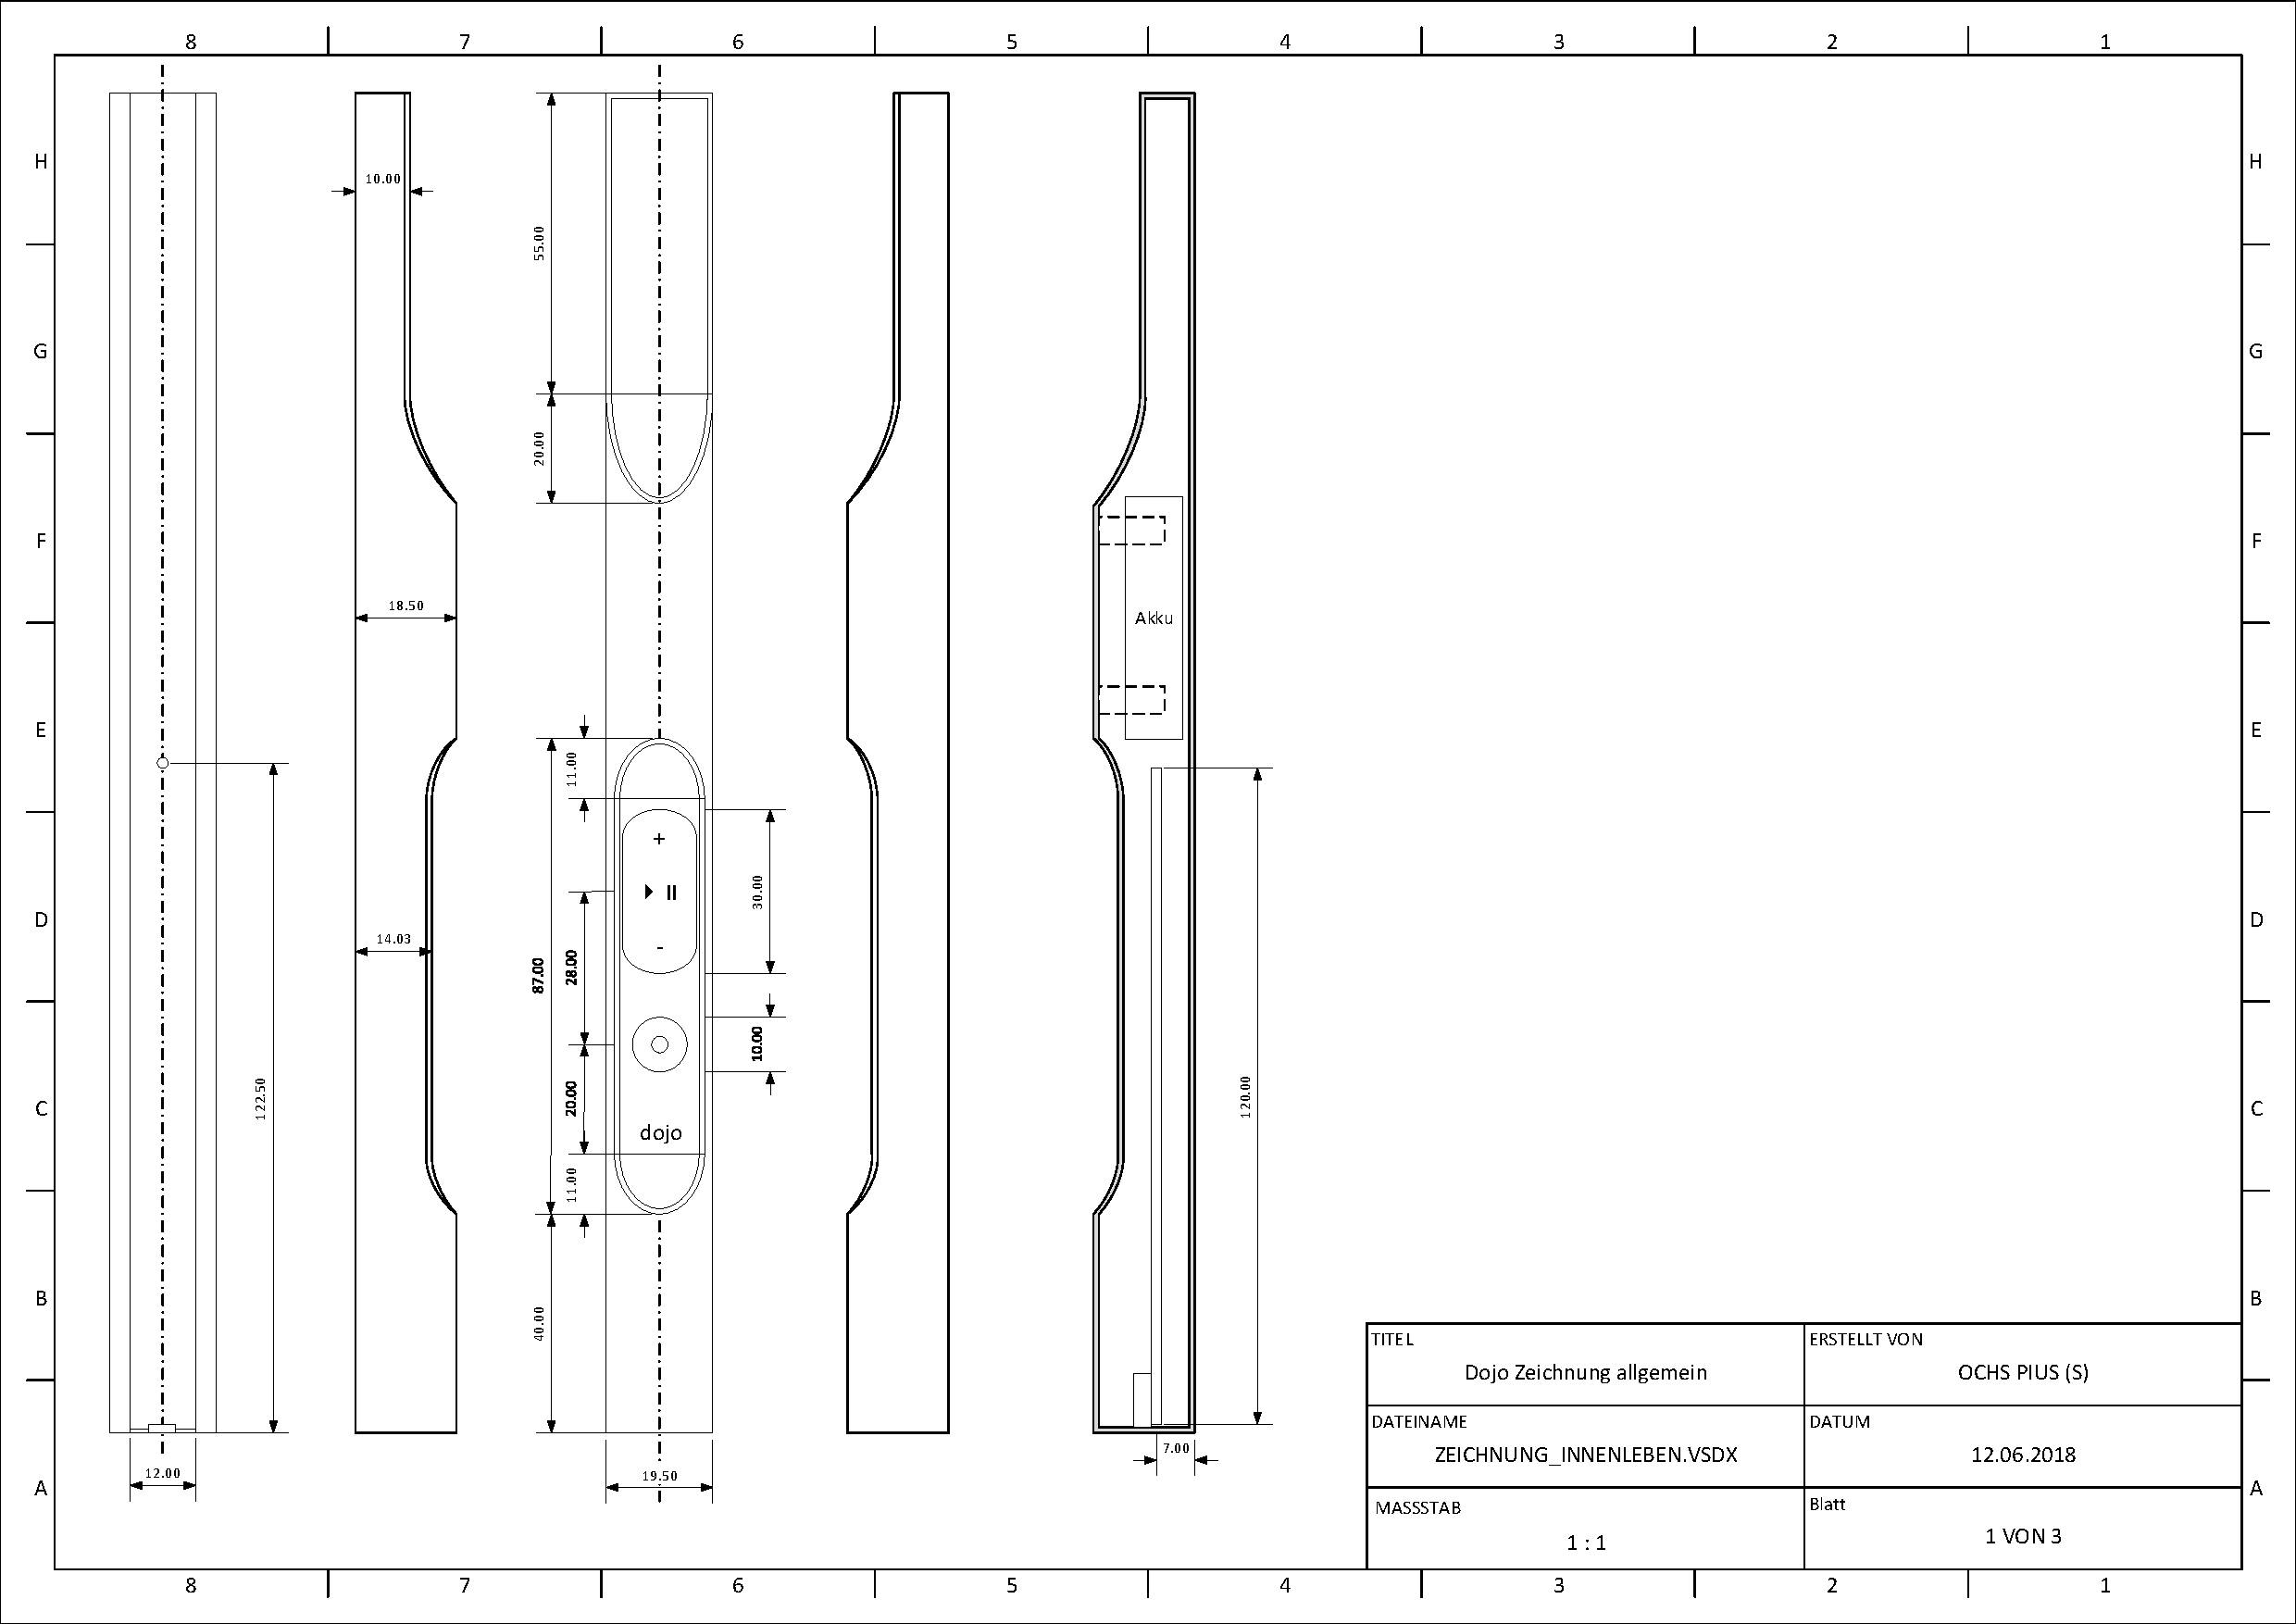
\includepdf[fitpaper]{Aufbau1.pdf}

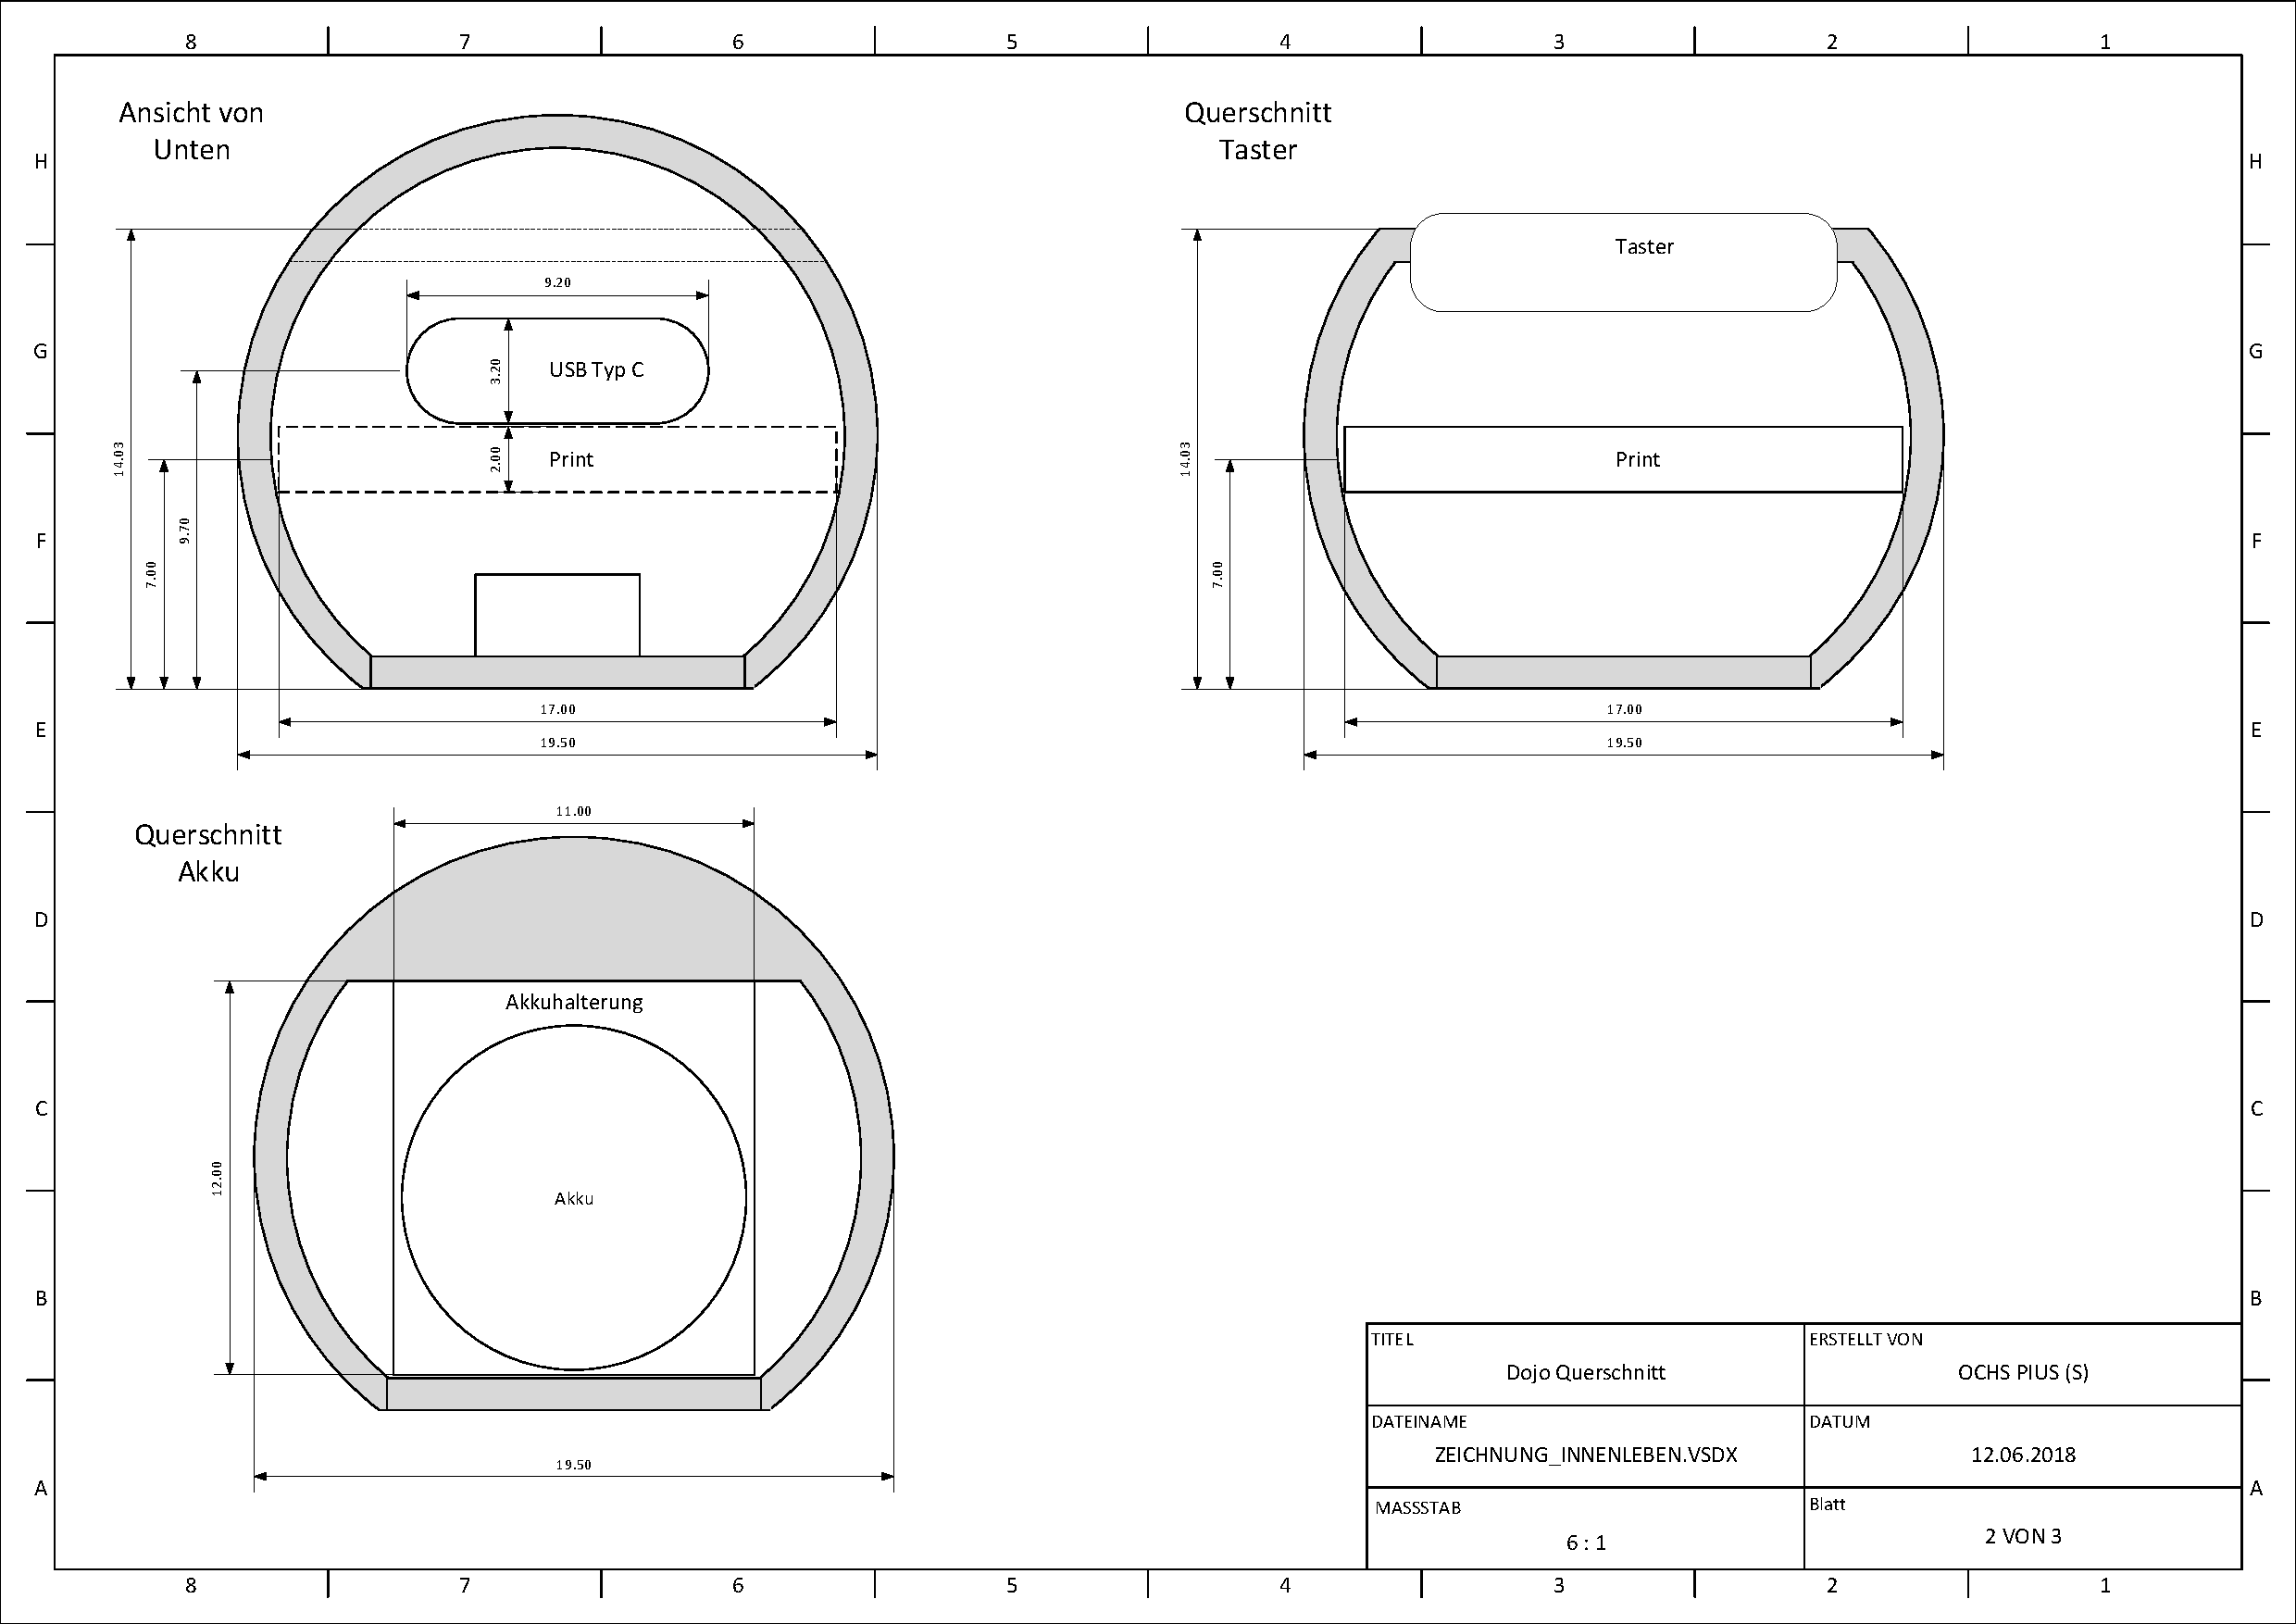
\includepdf[fitpaper]{Aufbau2.pdf}

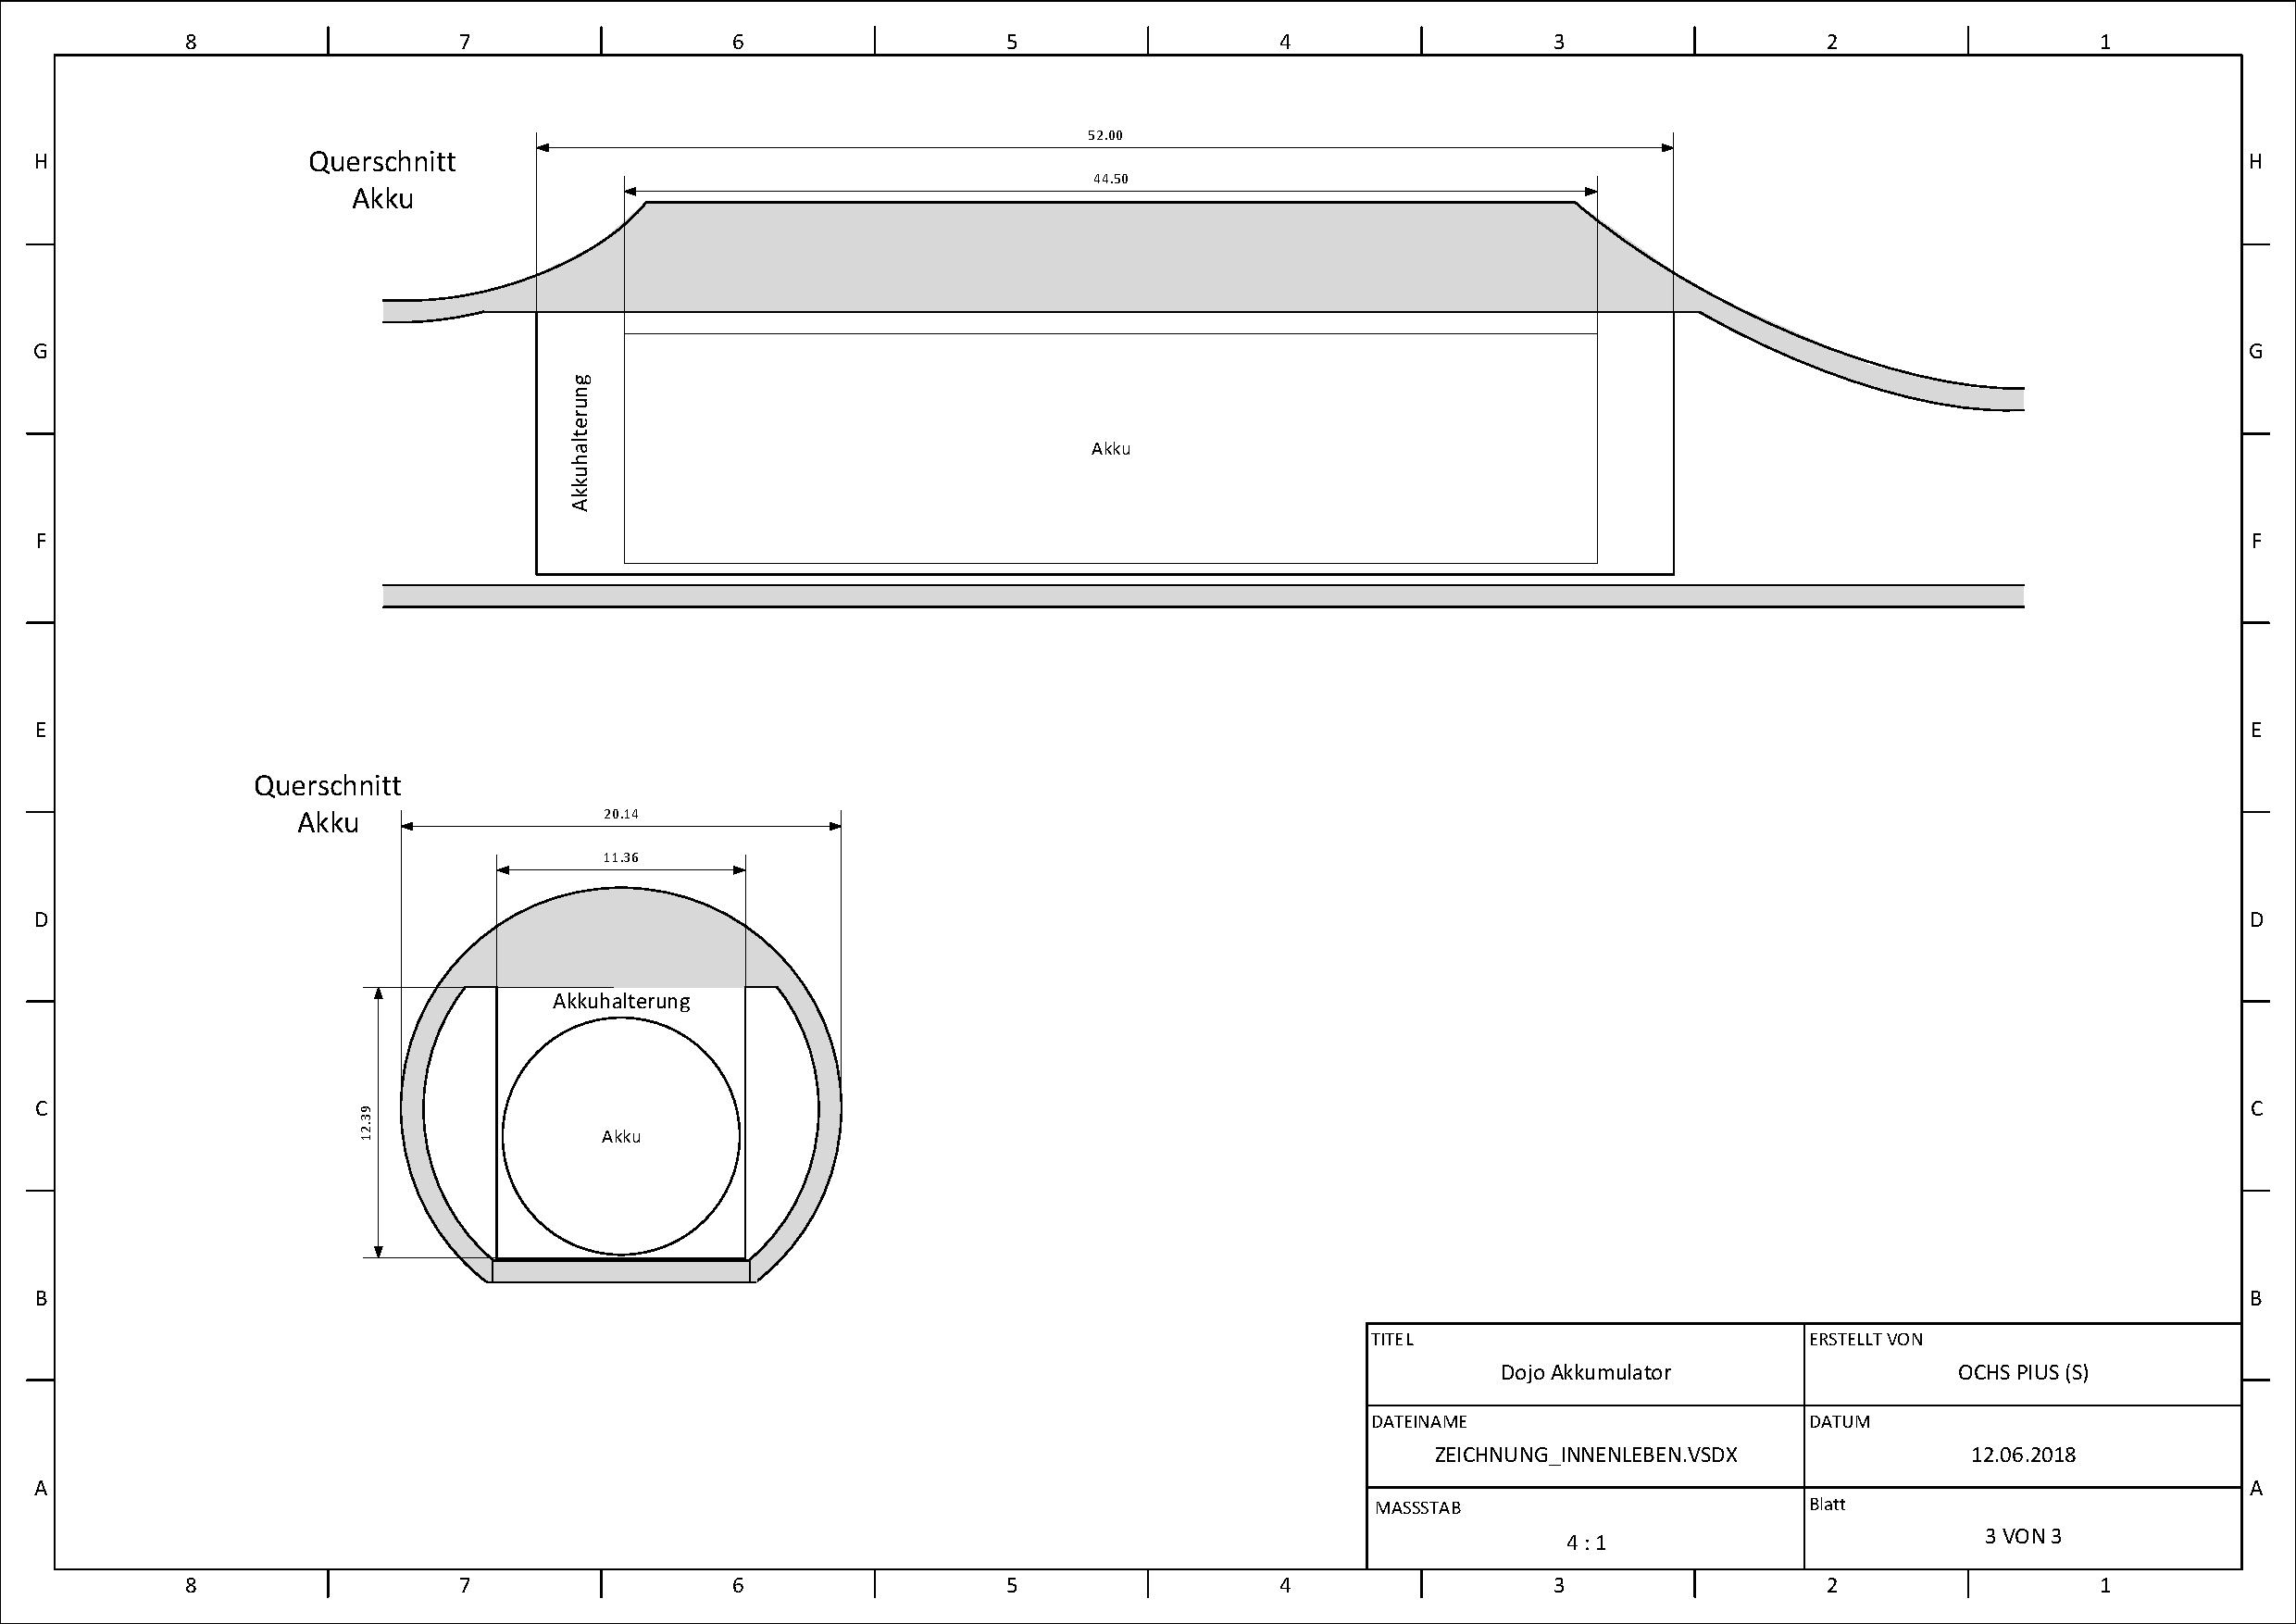
\includepdf[fitpaper]{Aufbau3.pdf}


\section{Prototyp 1}
\label{Prototyp 1}

\subsection*{Top}
\begin{figure}[htb]
\begin{center}
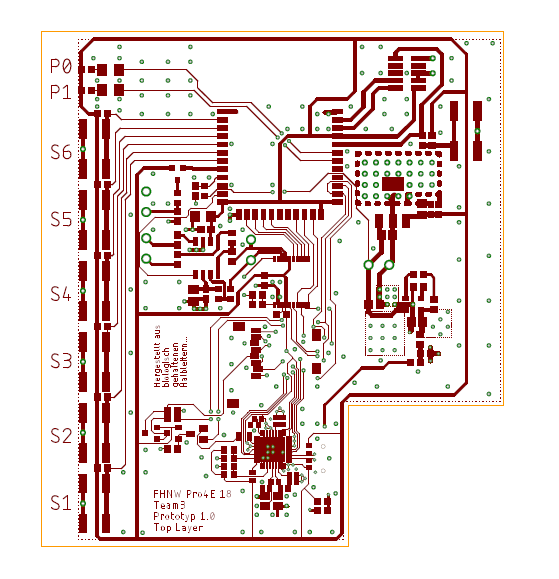
\includegraphics[width=\textwidth]{Board_1_A1.png}
\end{center}
\end{figure}

\newpage
\subsection*{Bottom}
\begin{figure}[htb]
\begin{center}
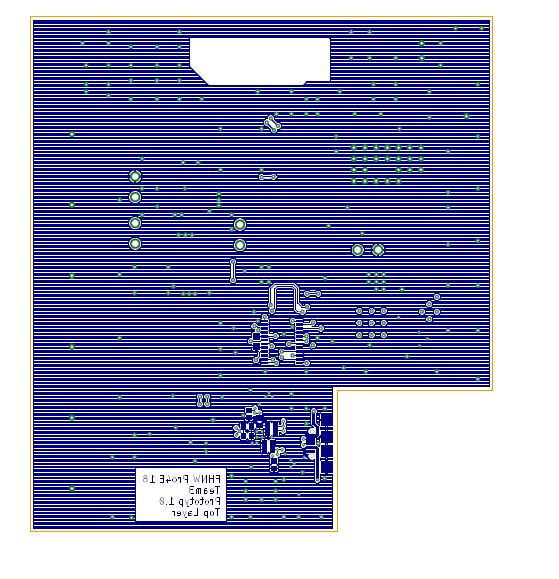
\includegraphics[width=\textwidth]{Board_1_B1.png}
\end{center}
\end{figure}

\newpage
\subsection*{Bestückung Bottom}
\begin{figure}[htb]
\begin{center}
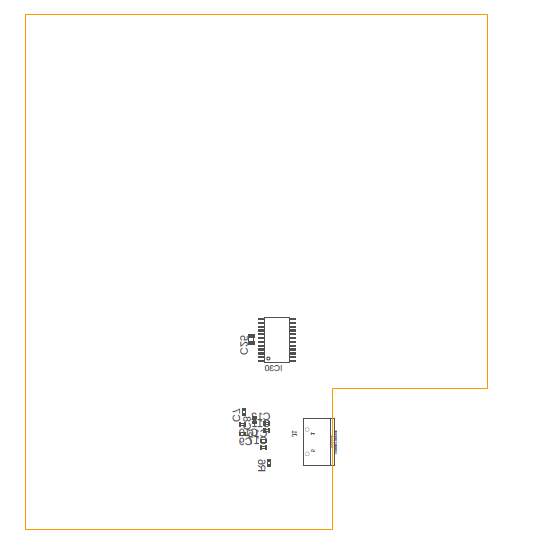
\includegraphics[width=\textwidth]{Board_1_Best_bottom.png}
\end{center}
\end{figure}

\newpage
\subsection*{Bestückung Top}
\begin{figure}[htb]
\begin{center}
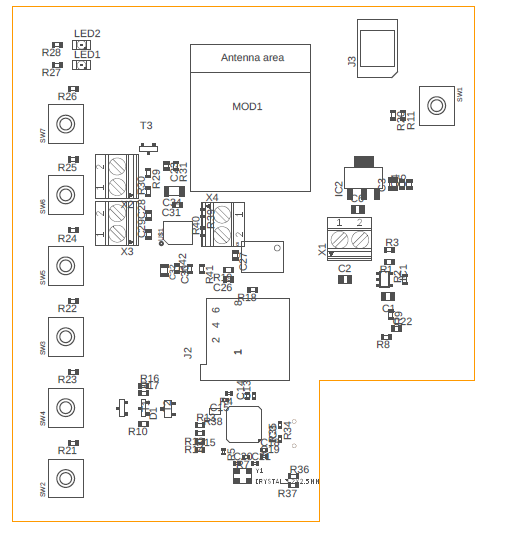
\includegraphics[width=\textwidth]{Board_1_Best_top.png}
\end{center}
\end{figure}

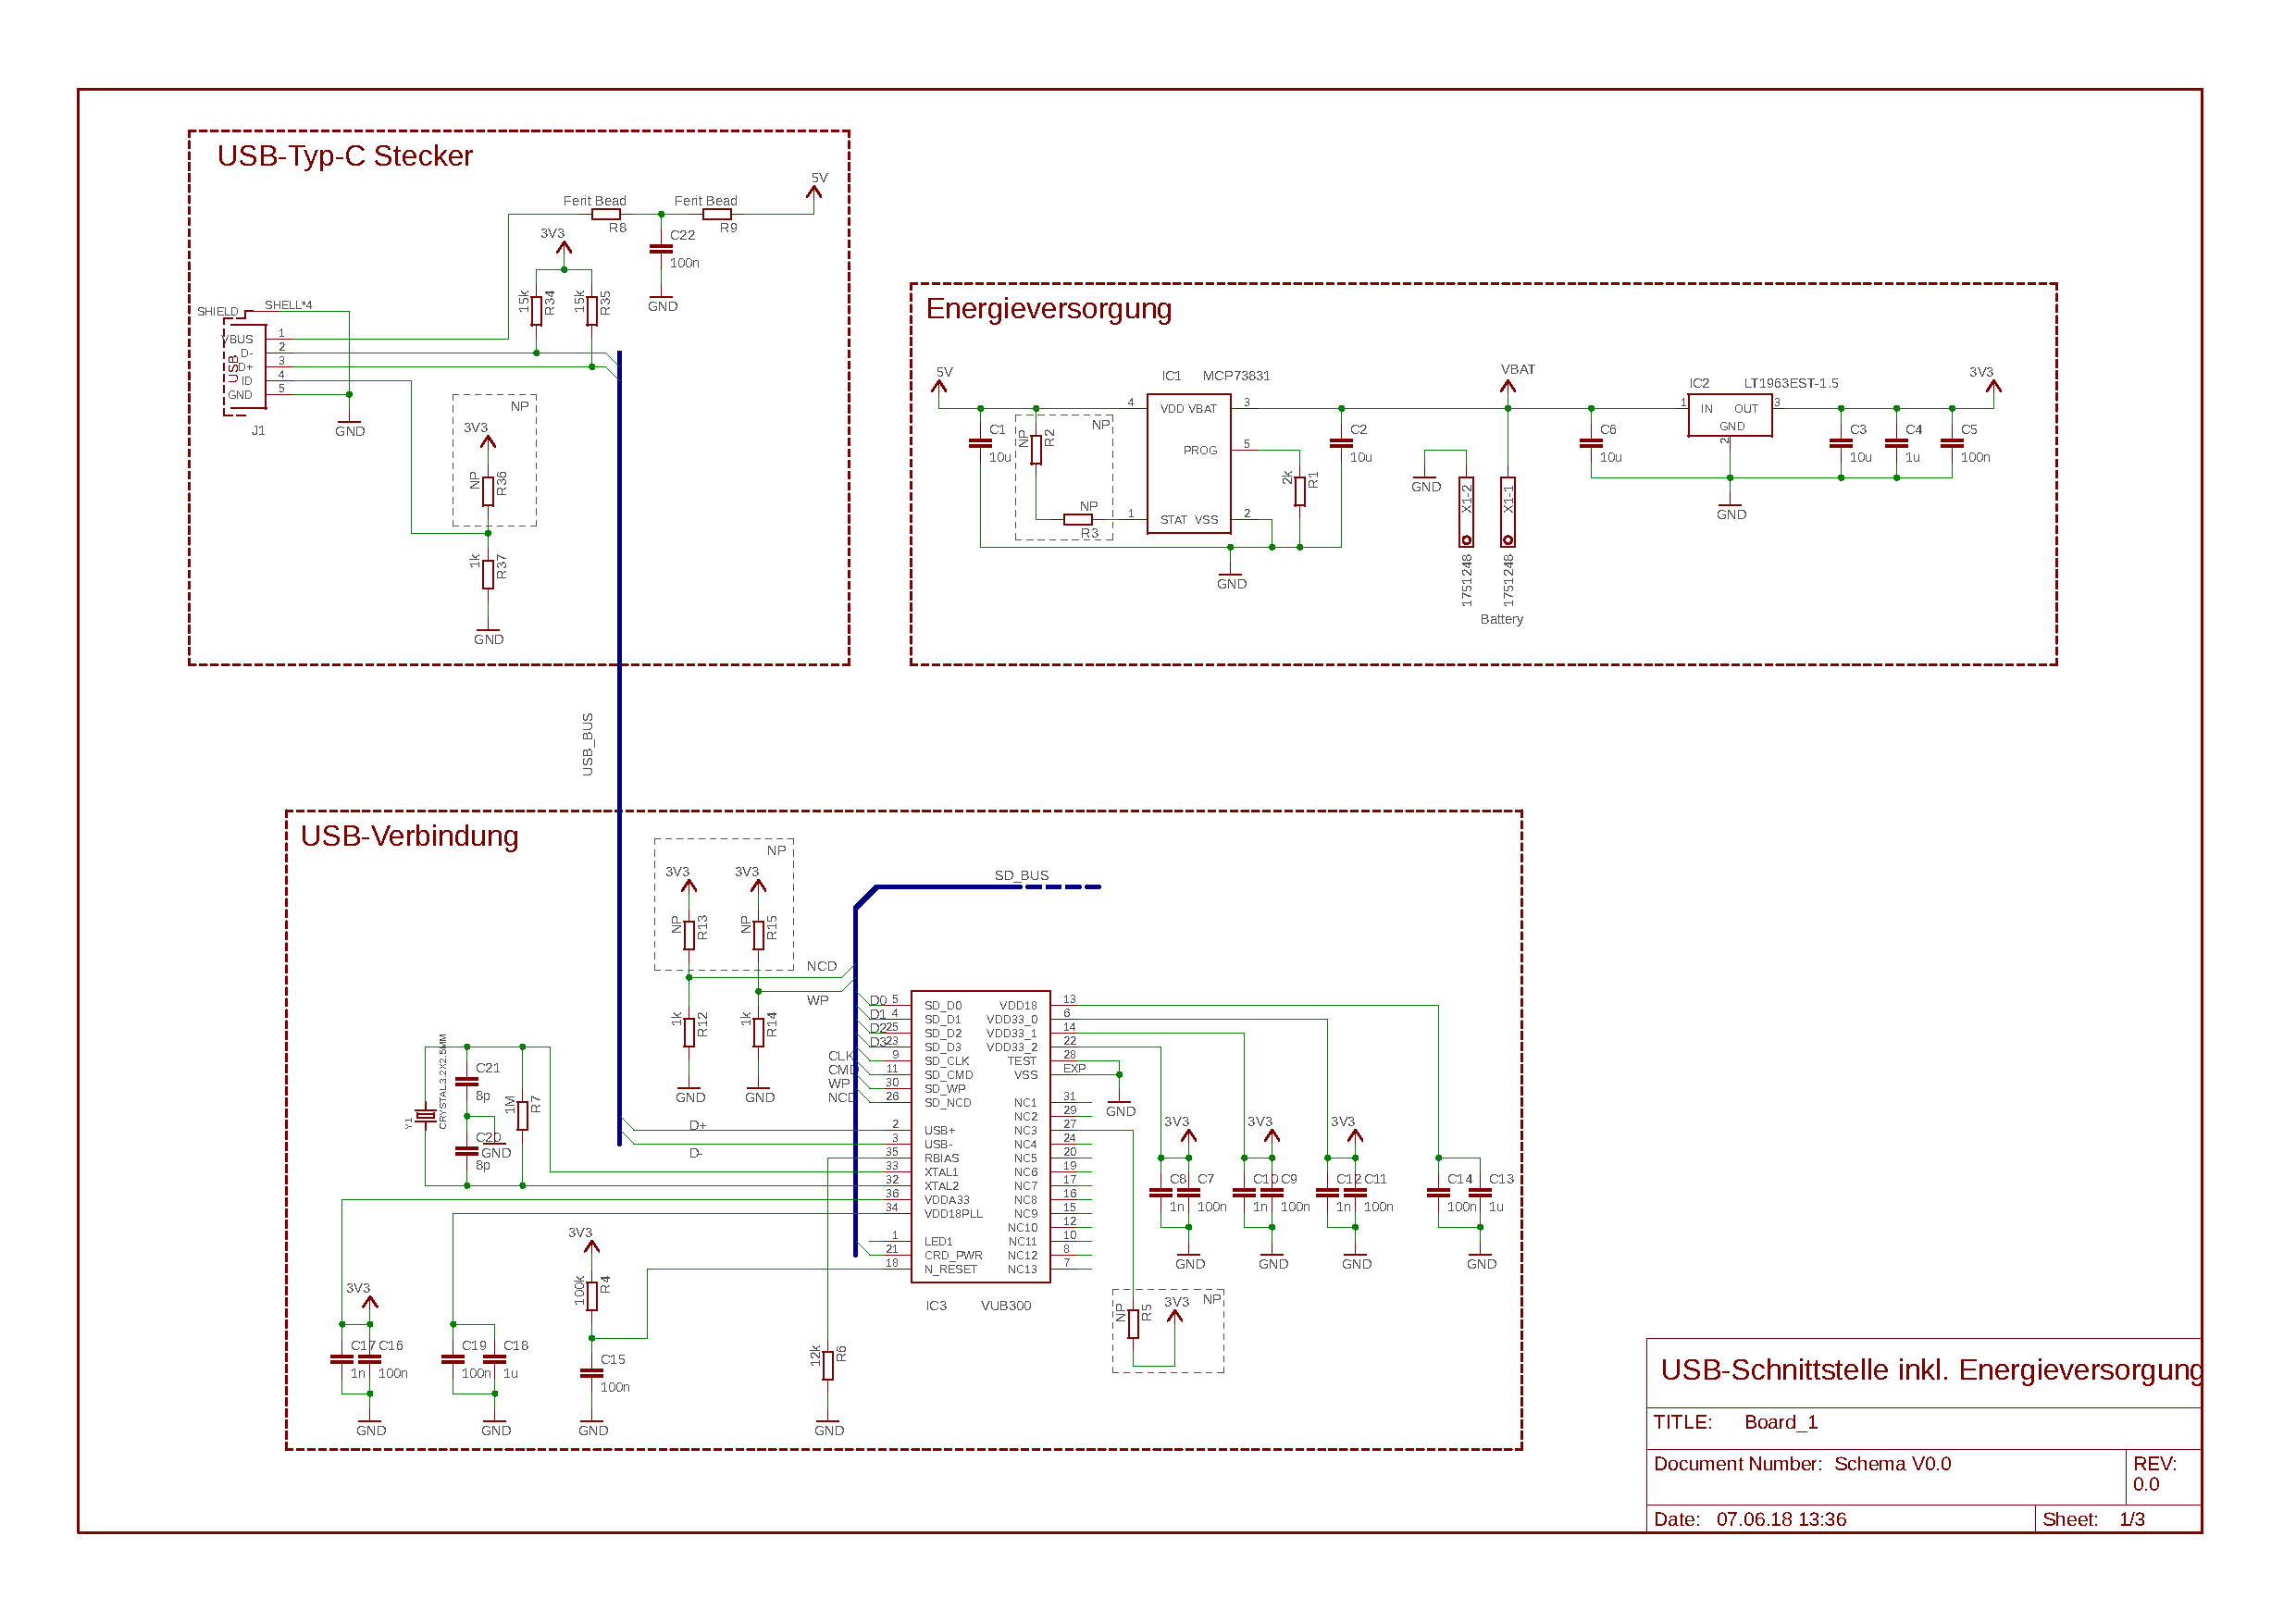
\includepdf[fitpaper]{Board_11.pdf}

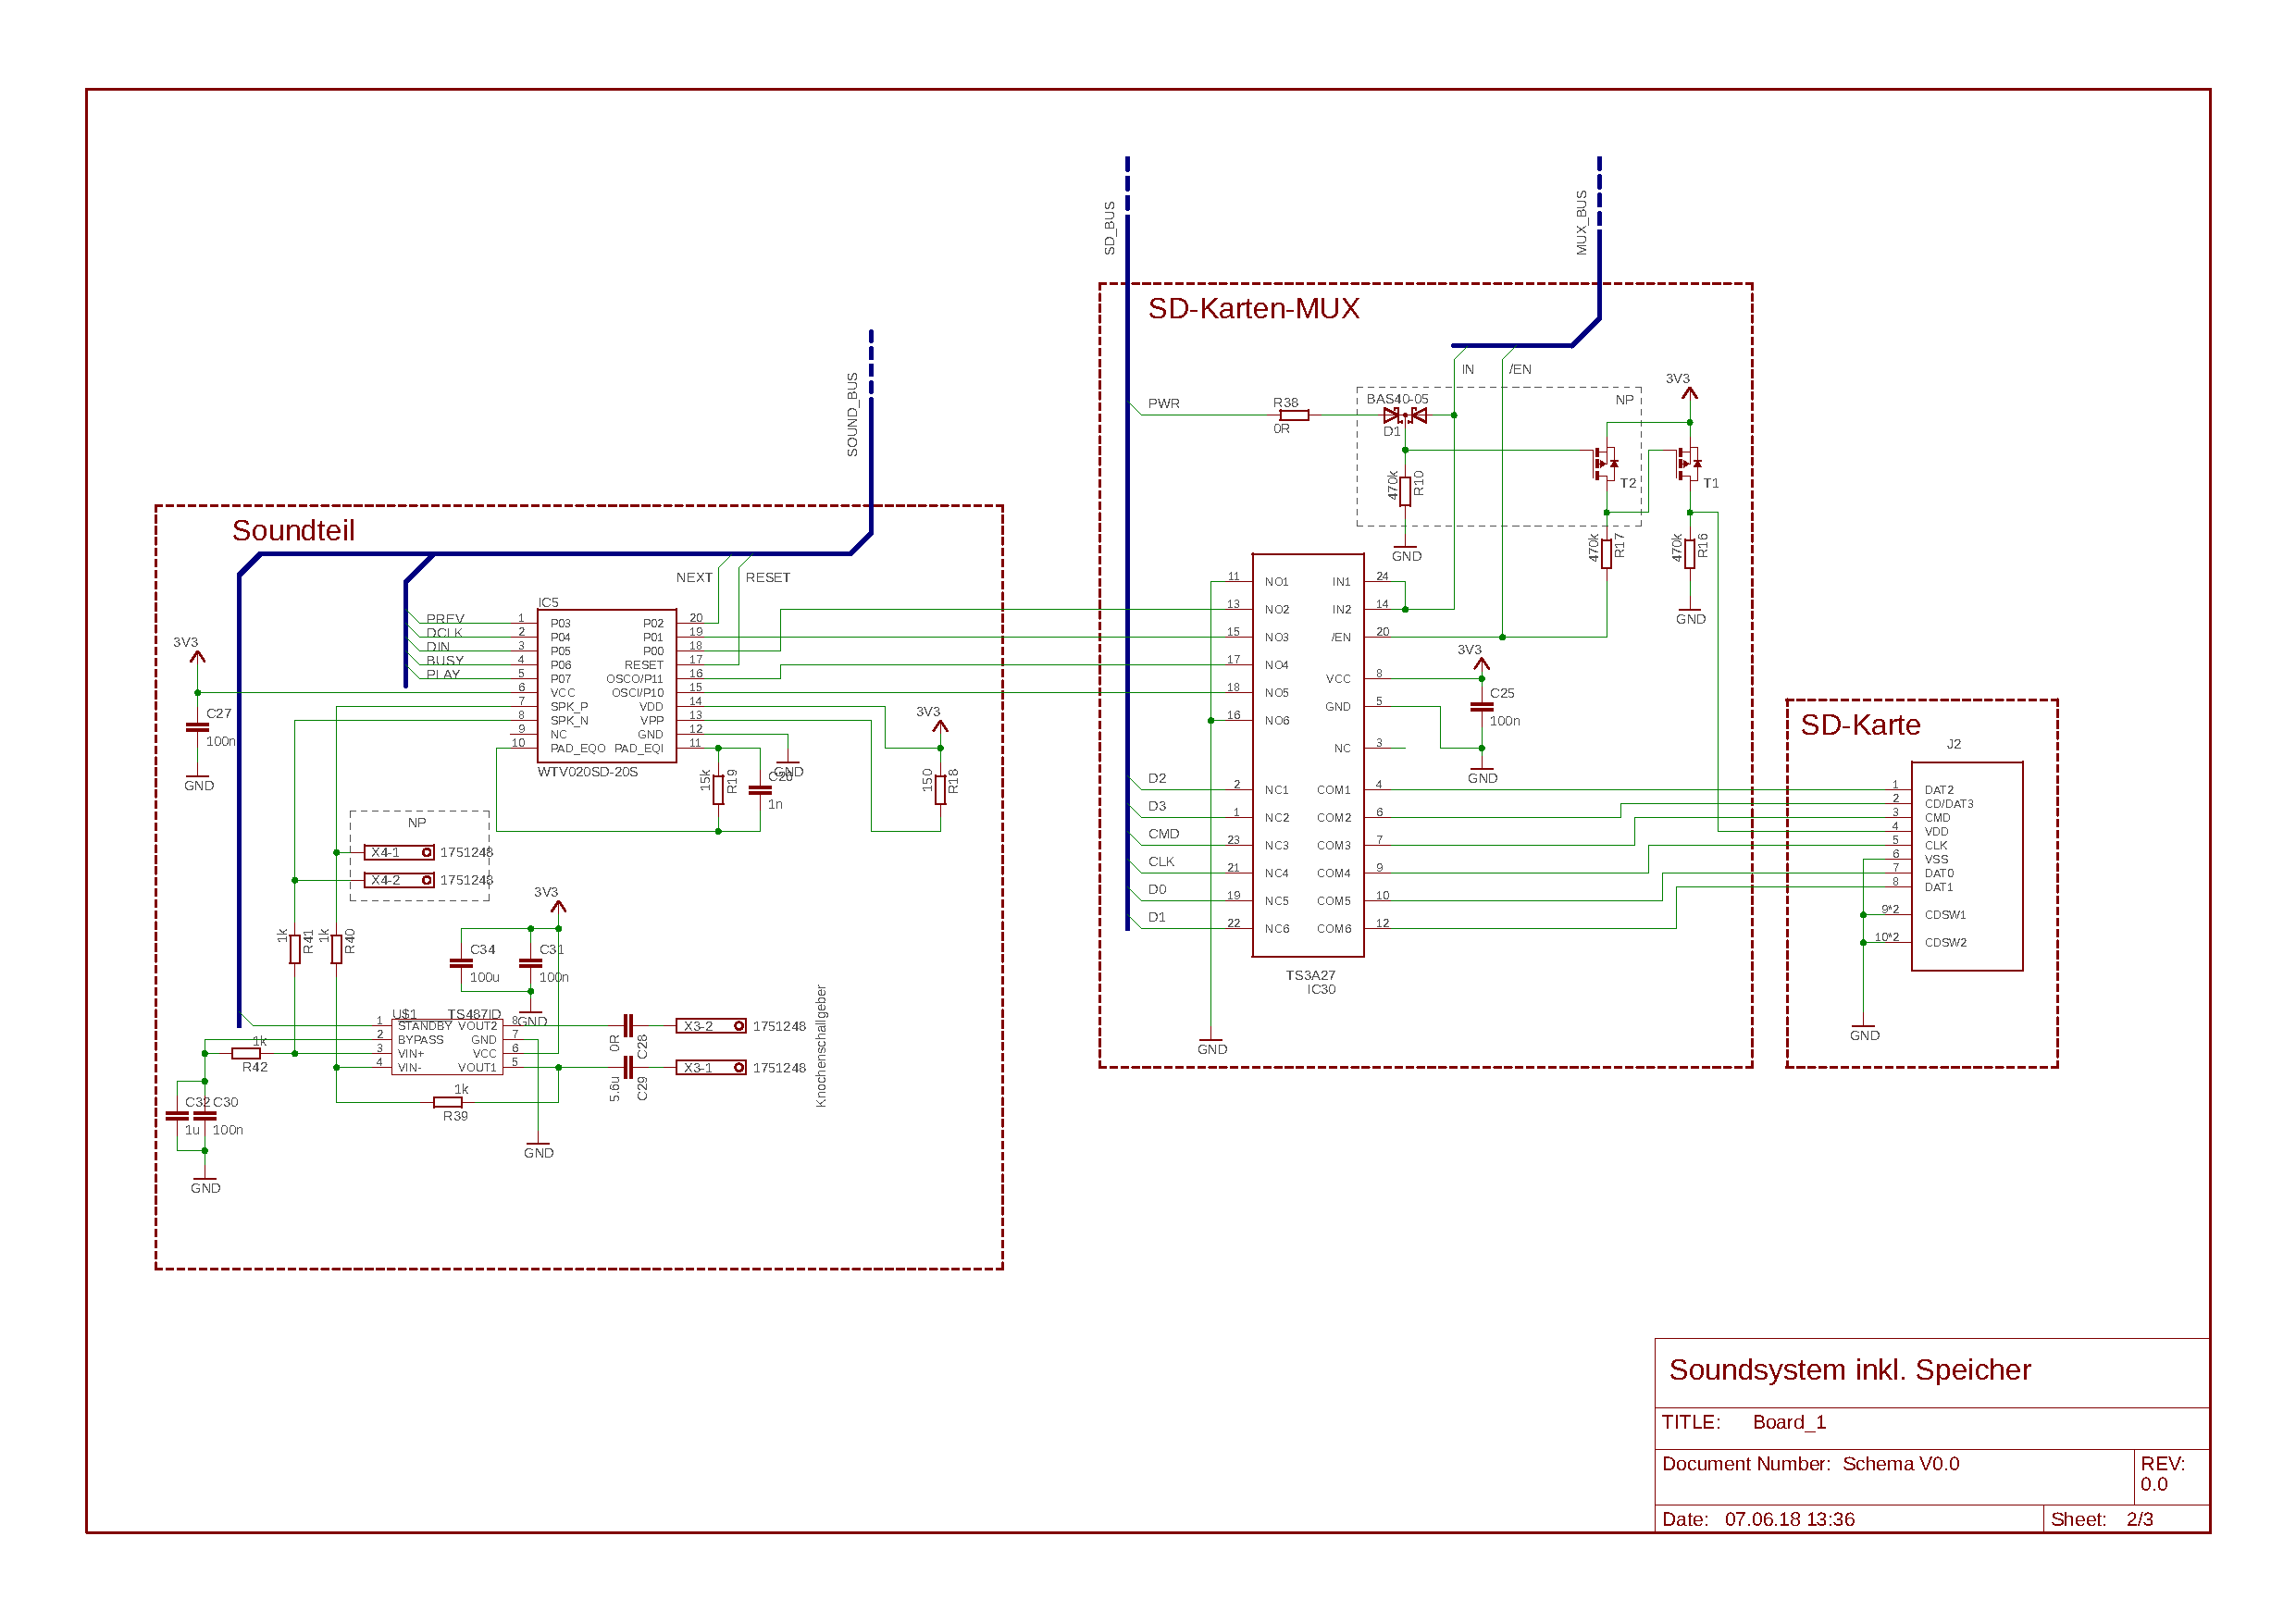
\includepdf[fitpaper]{Board_12.pdf}

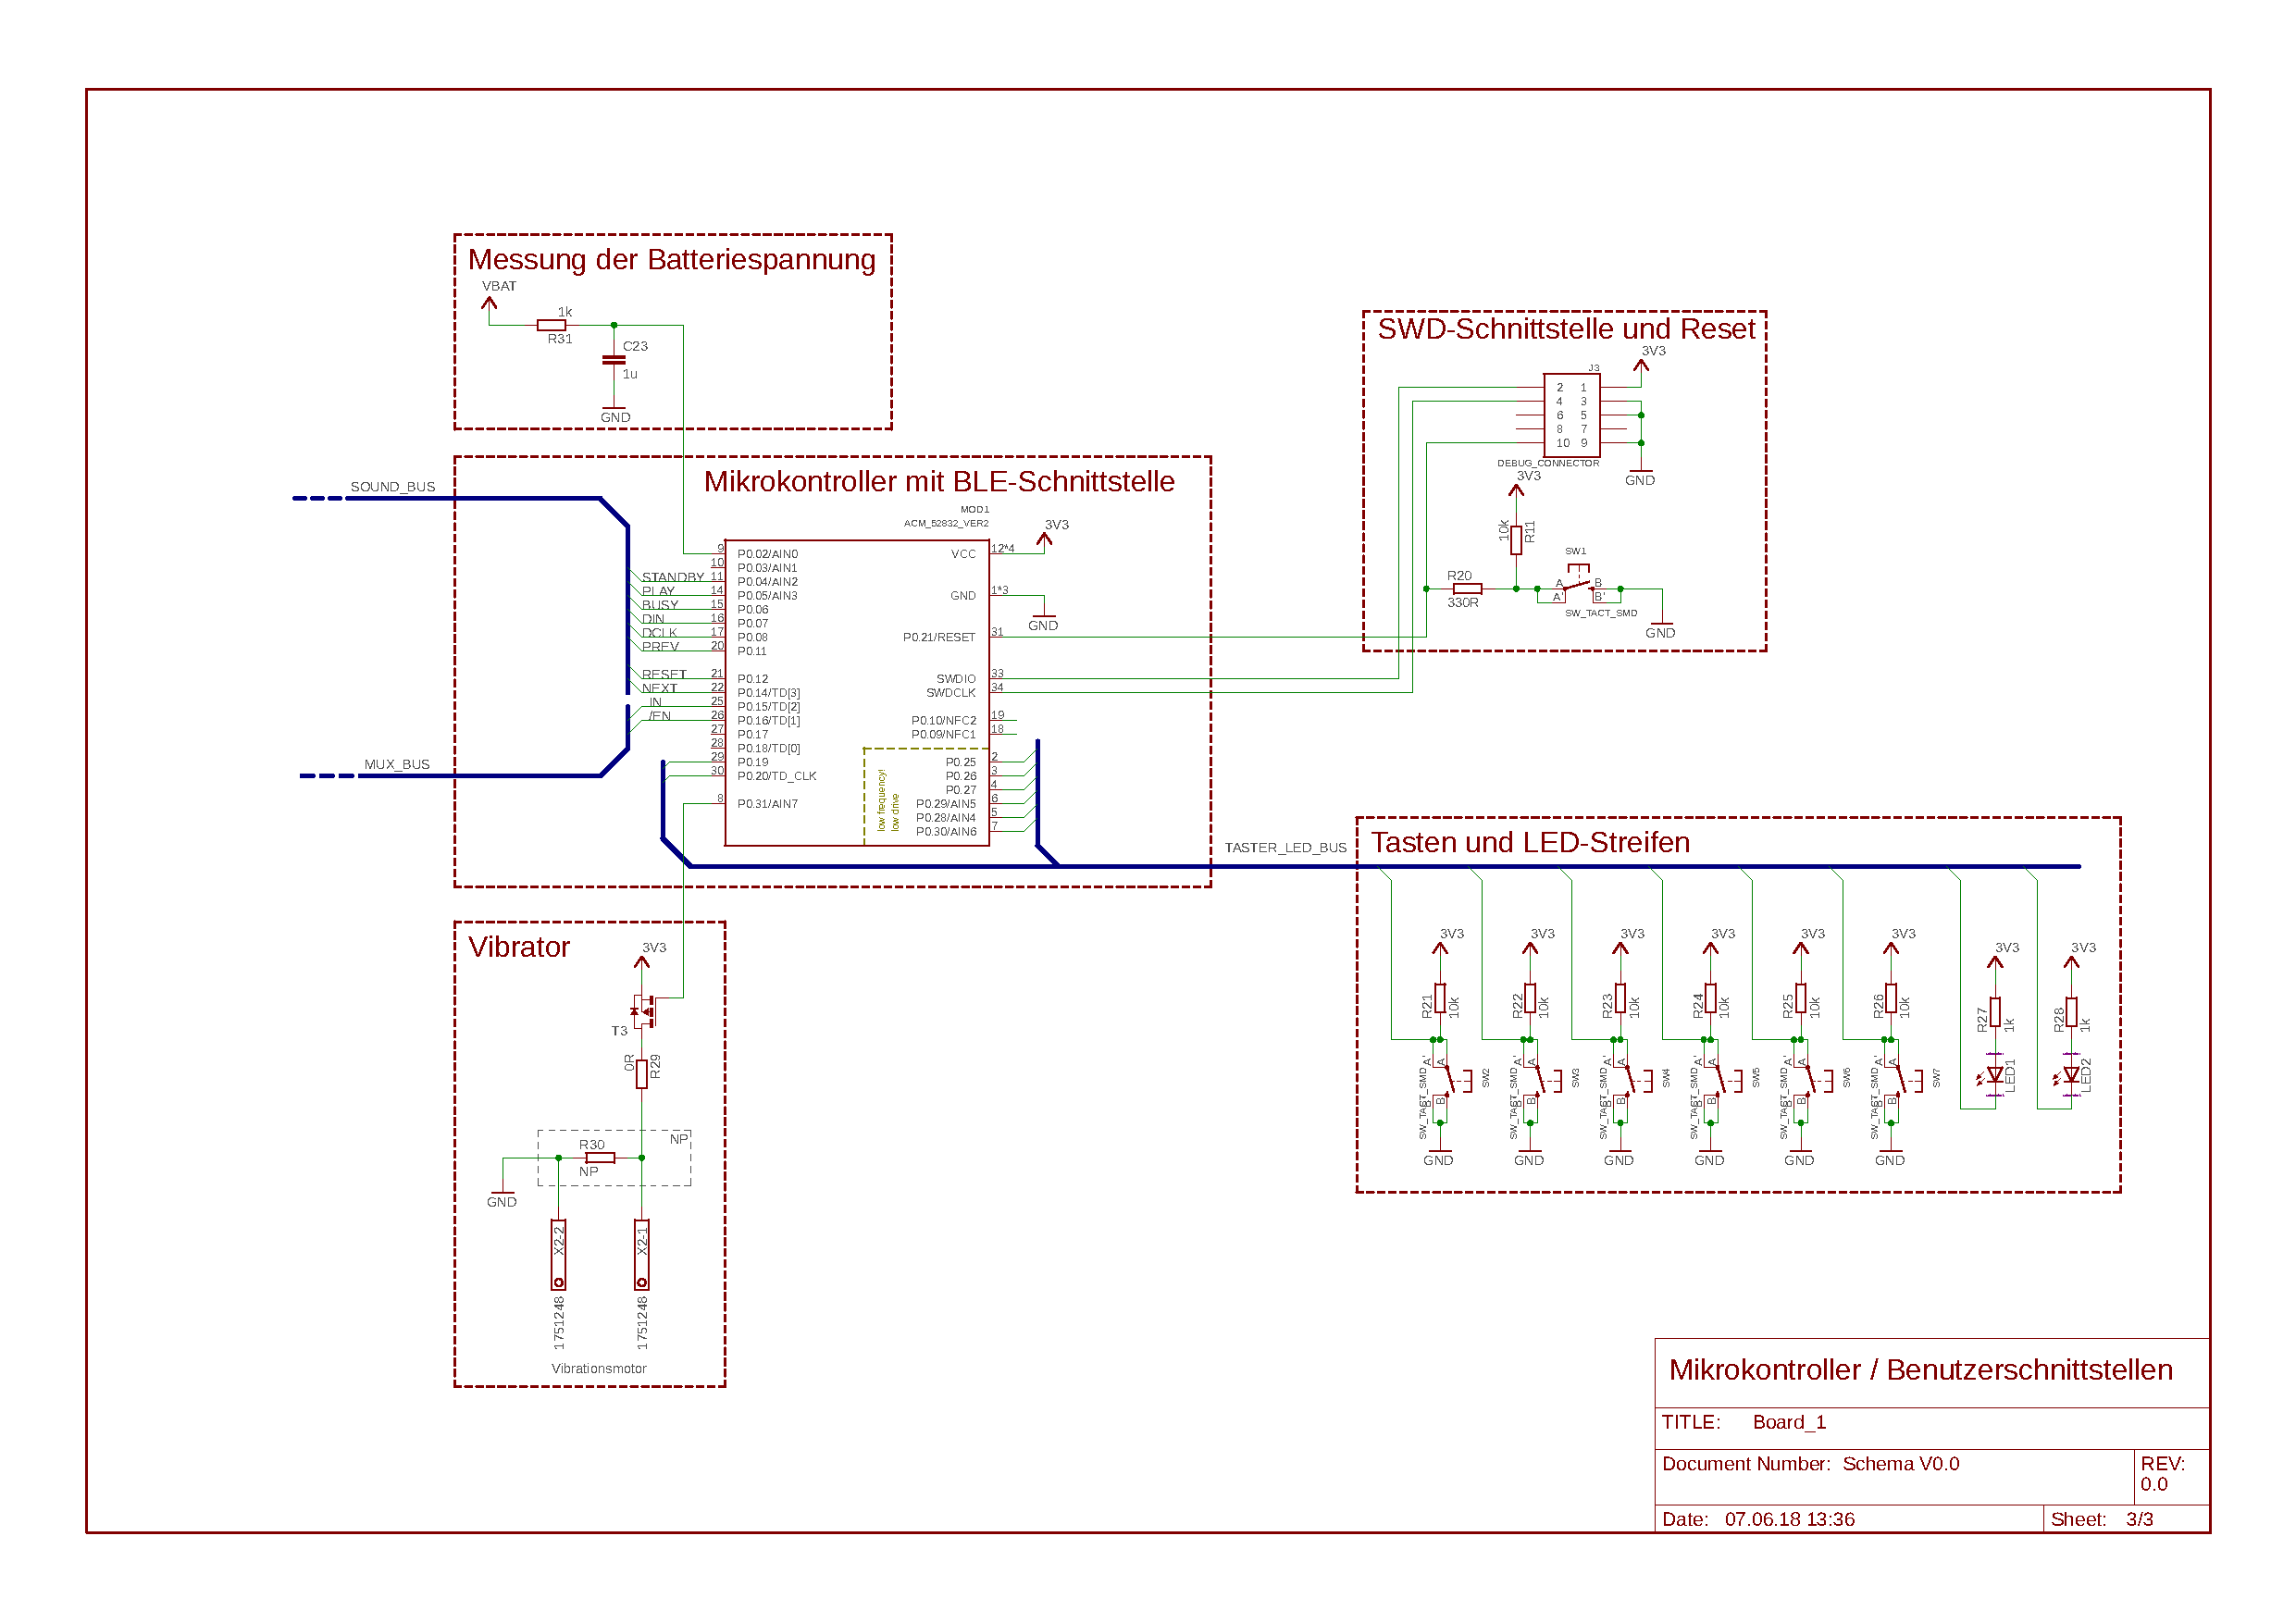
\includepdf[fitpaper]{Board_13.pdf}


\section{Prototyp 2}

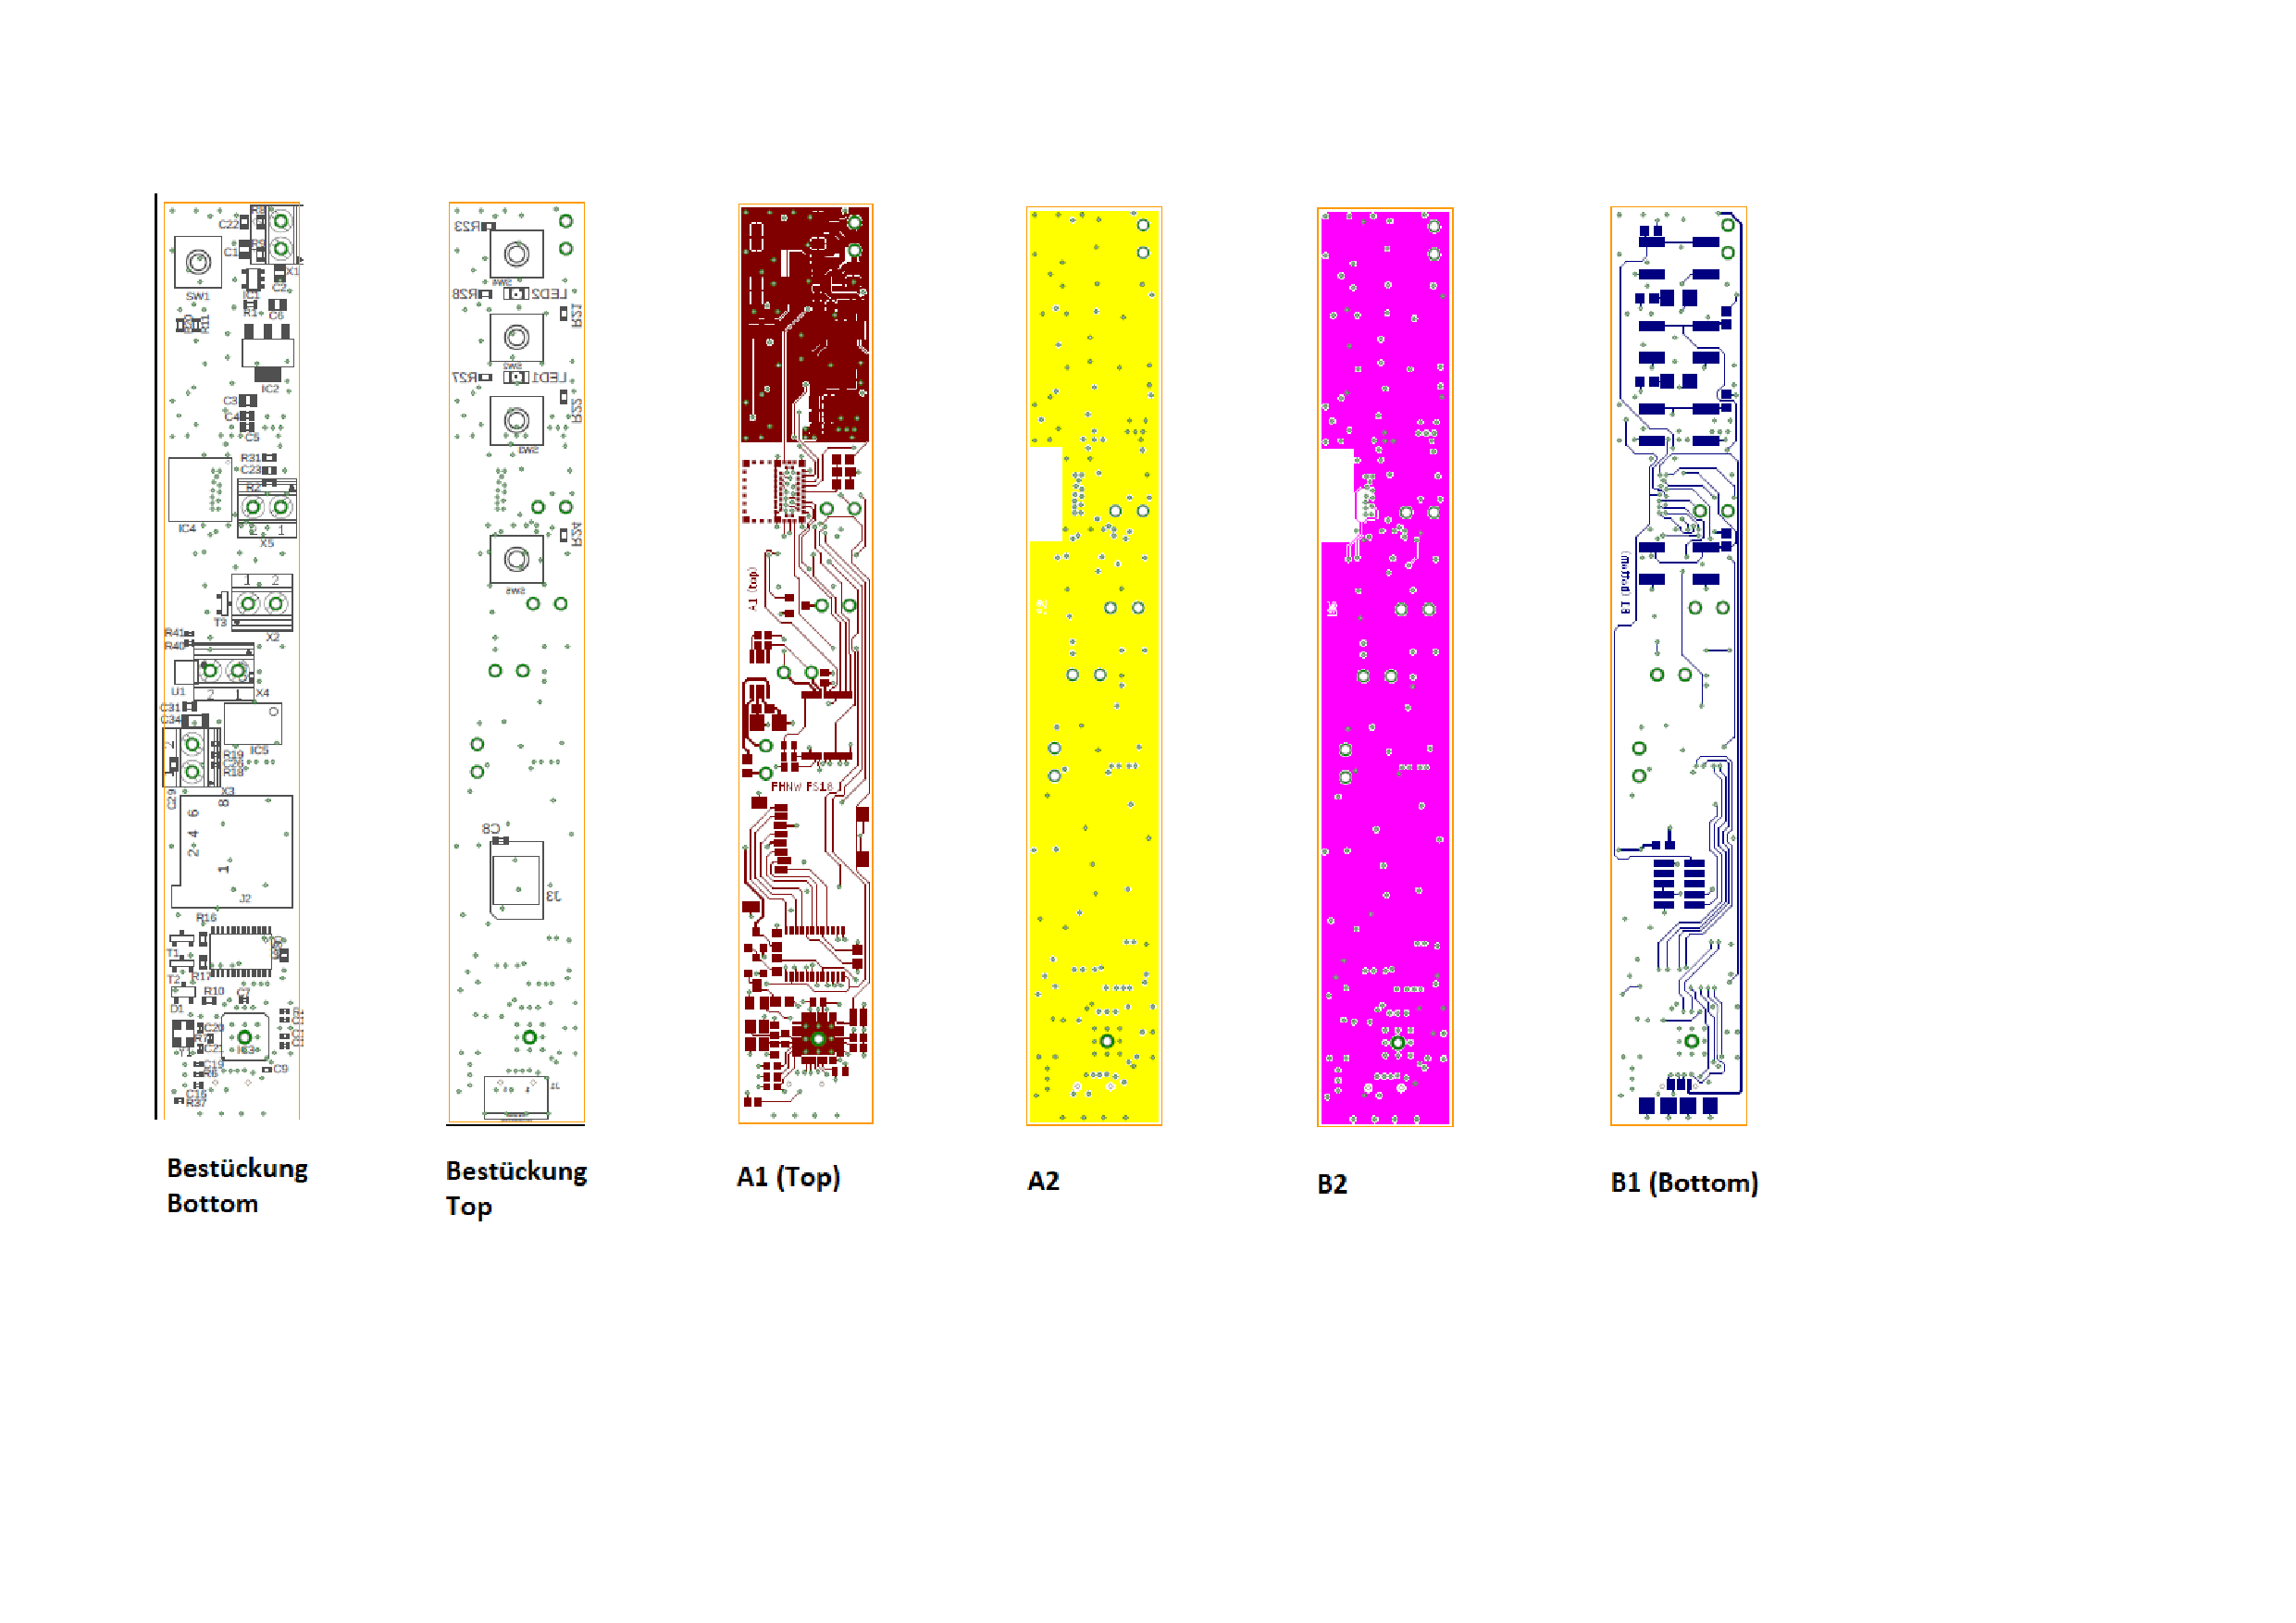
\includepdf[fitpaper]{dojo_layer.pdf}

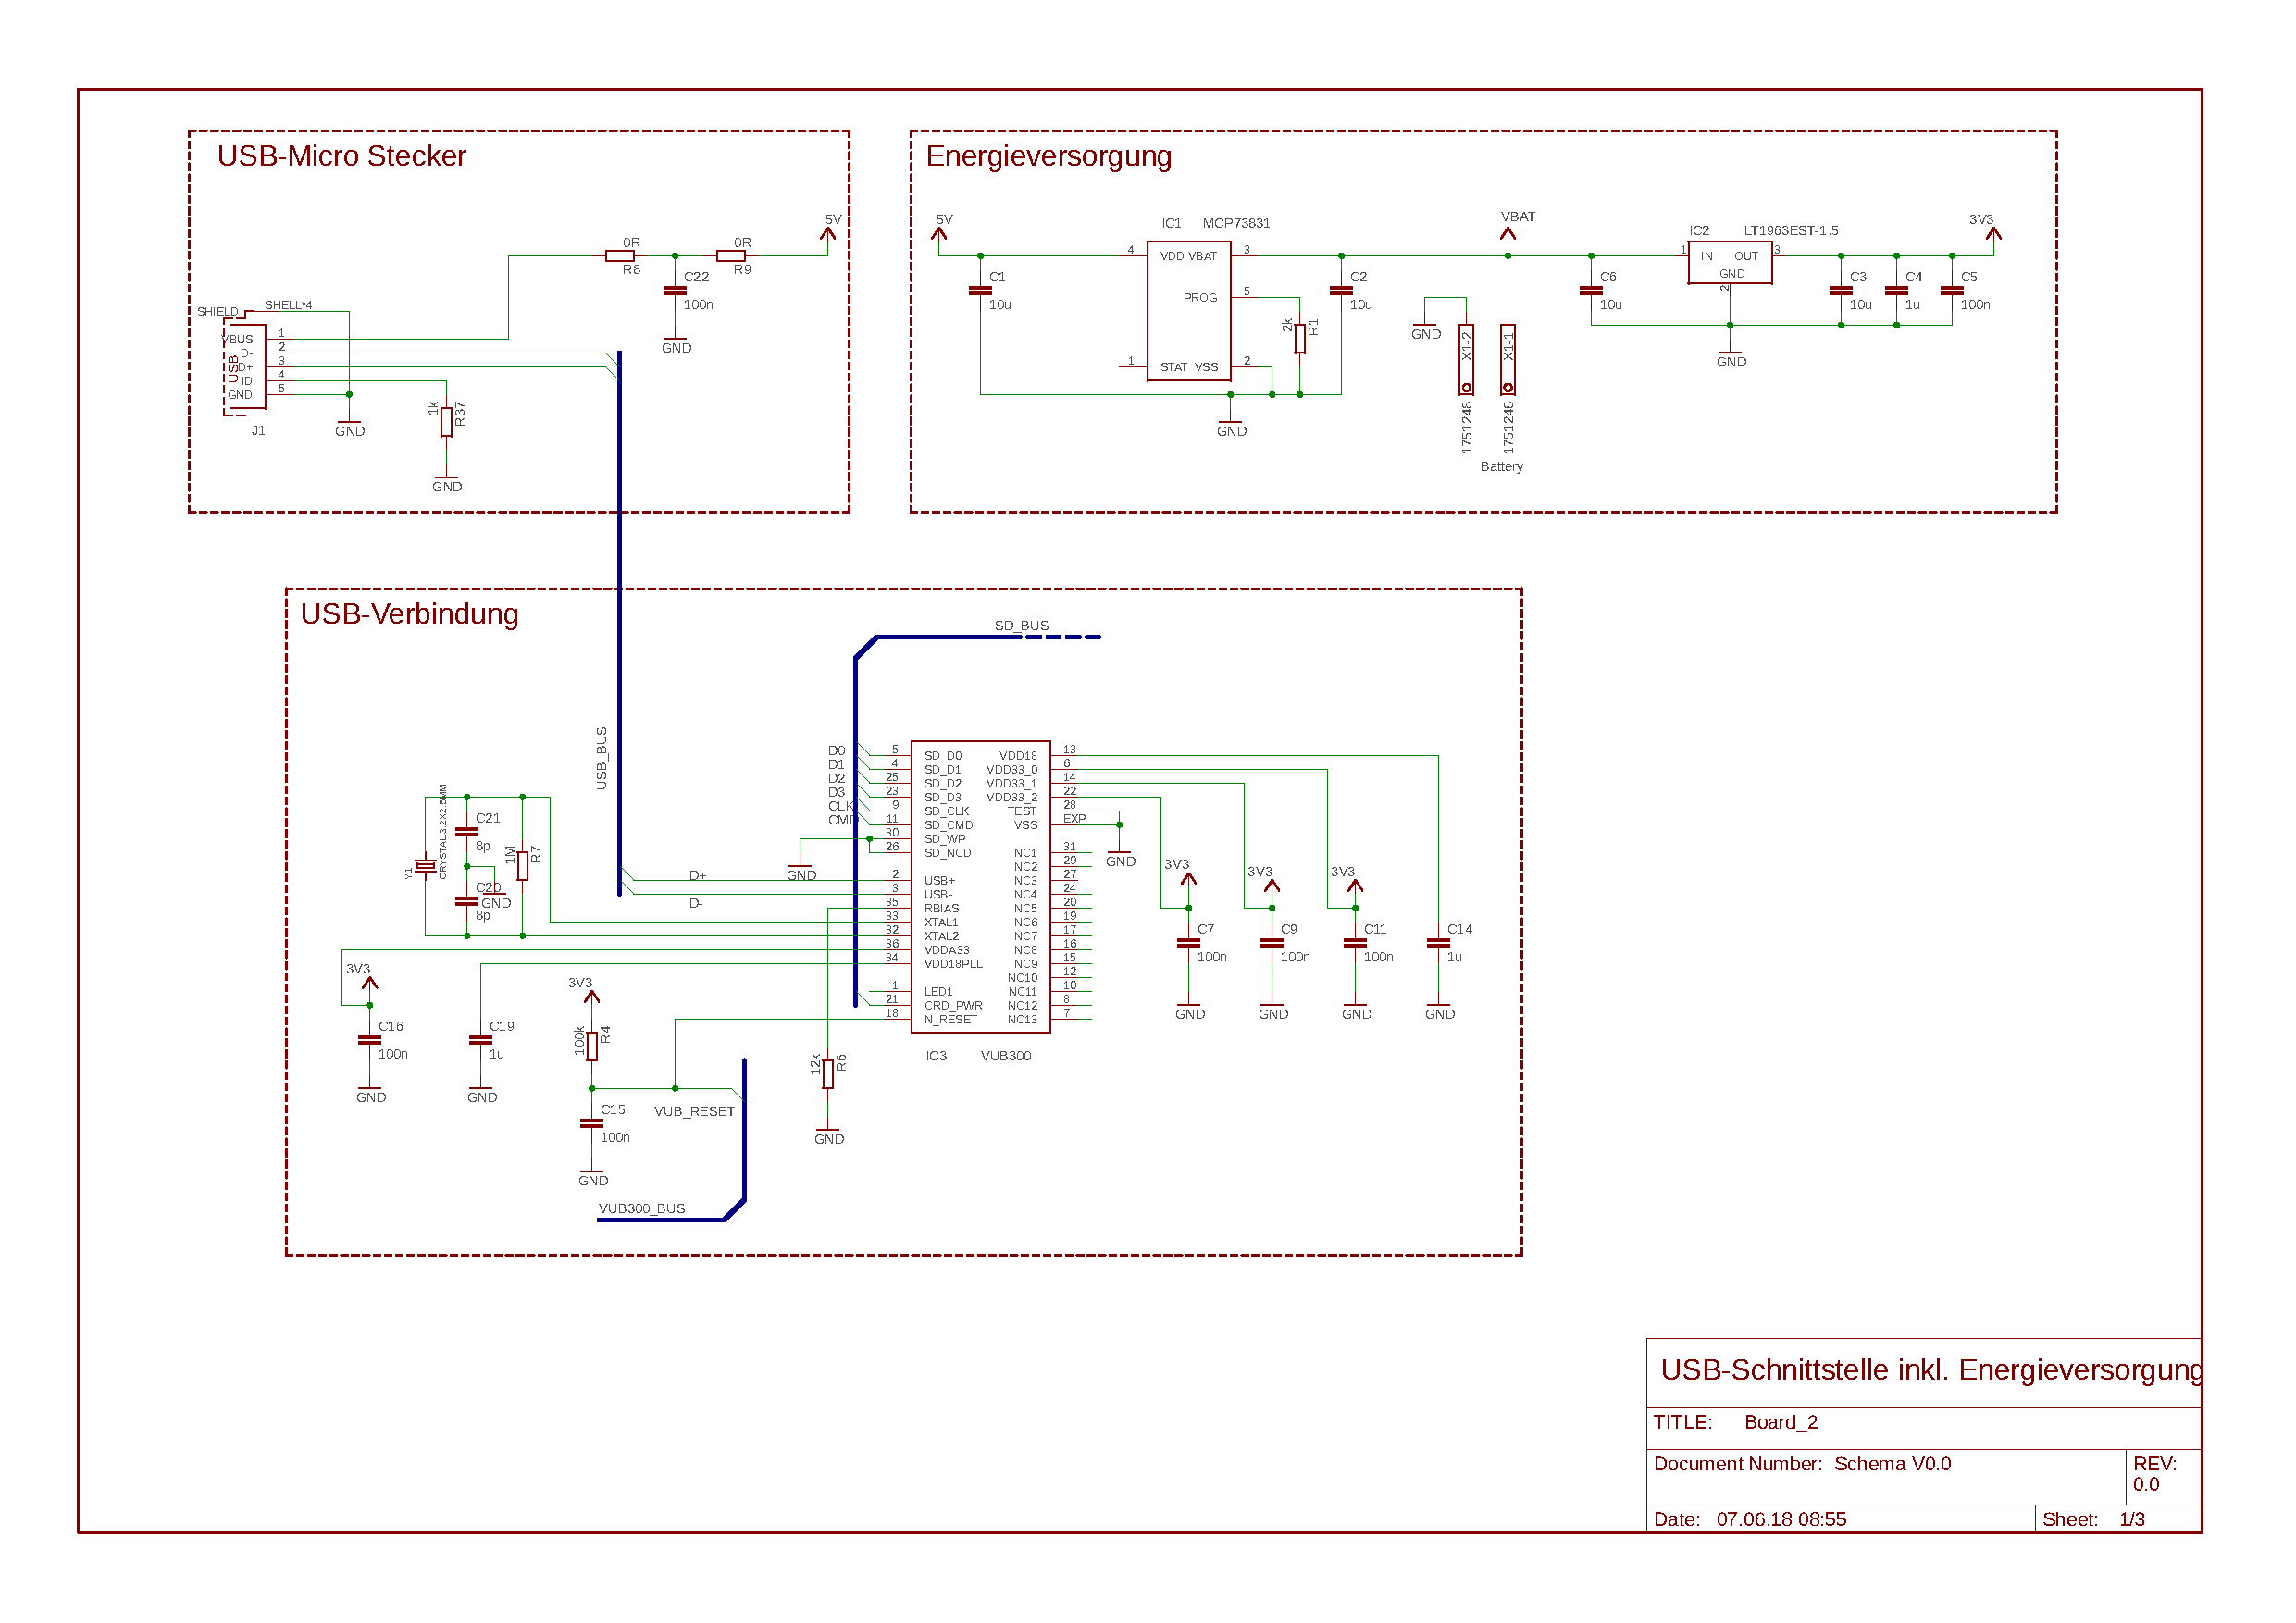
\includepdf[fitpaper]{Board_21.pdf}

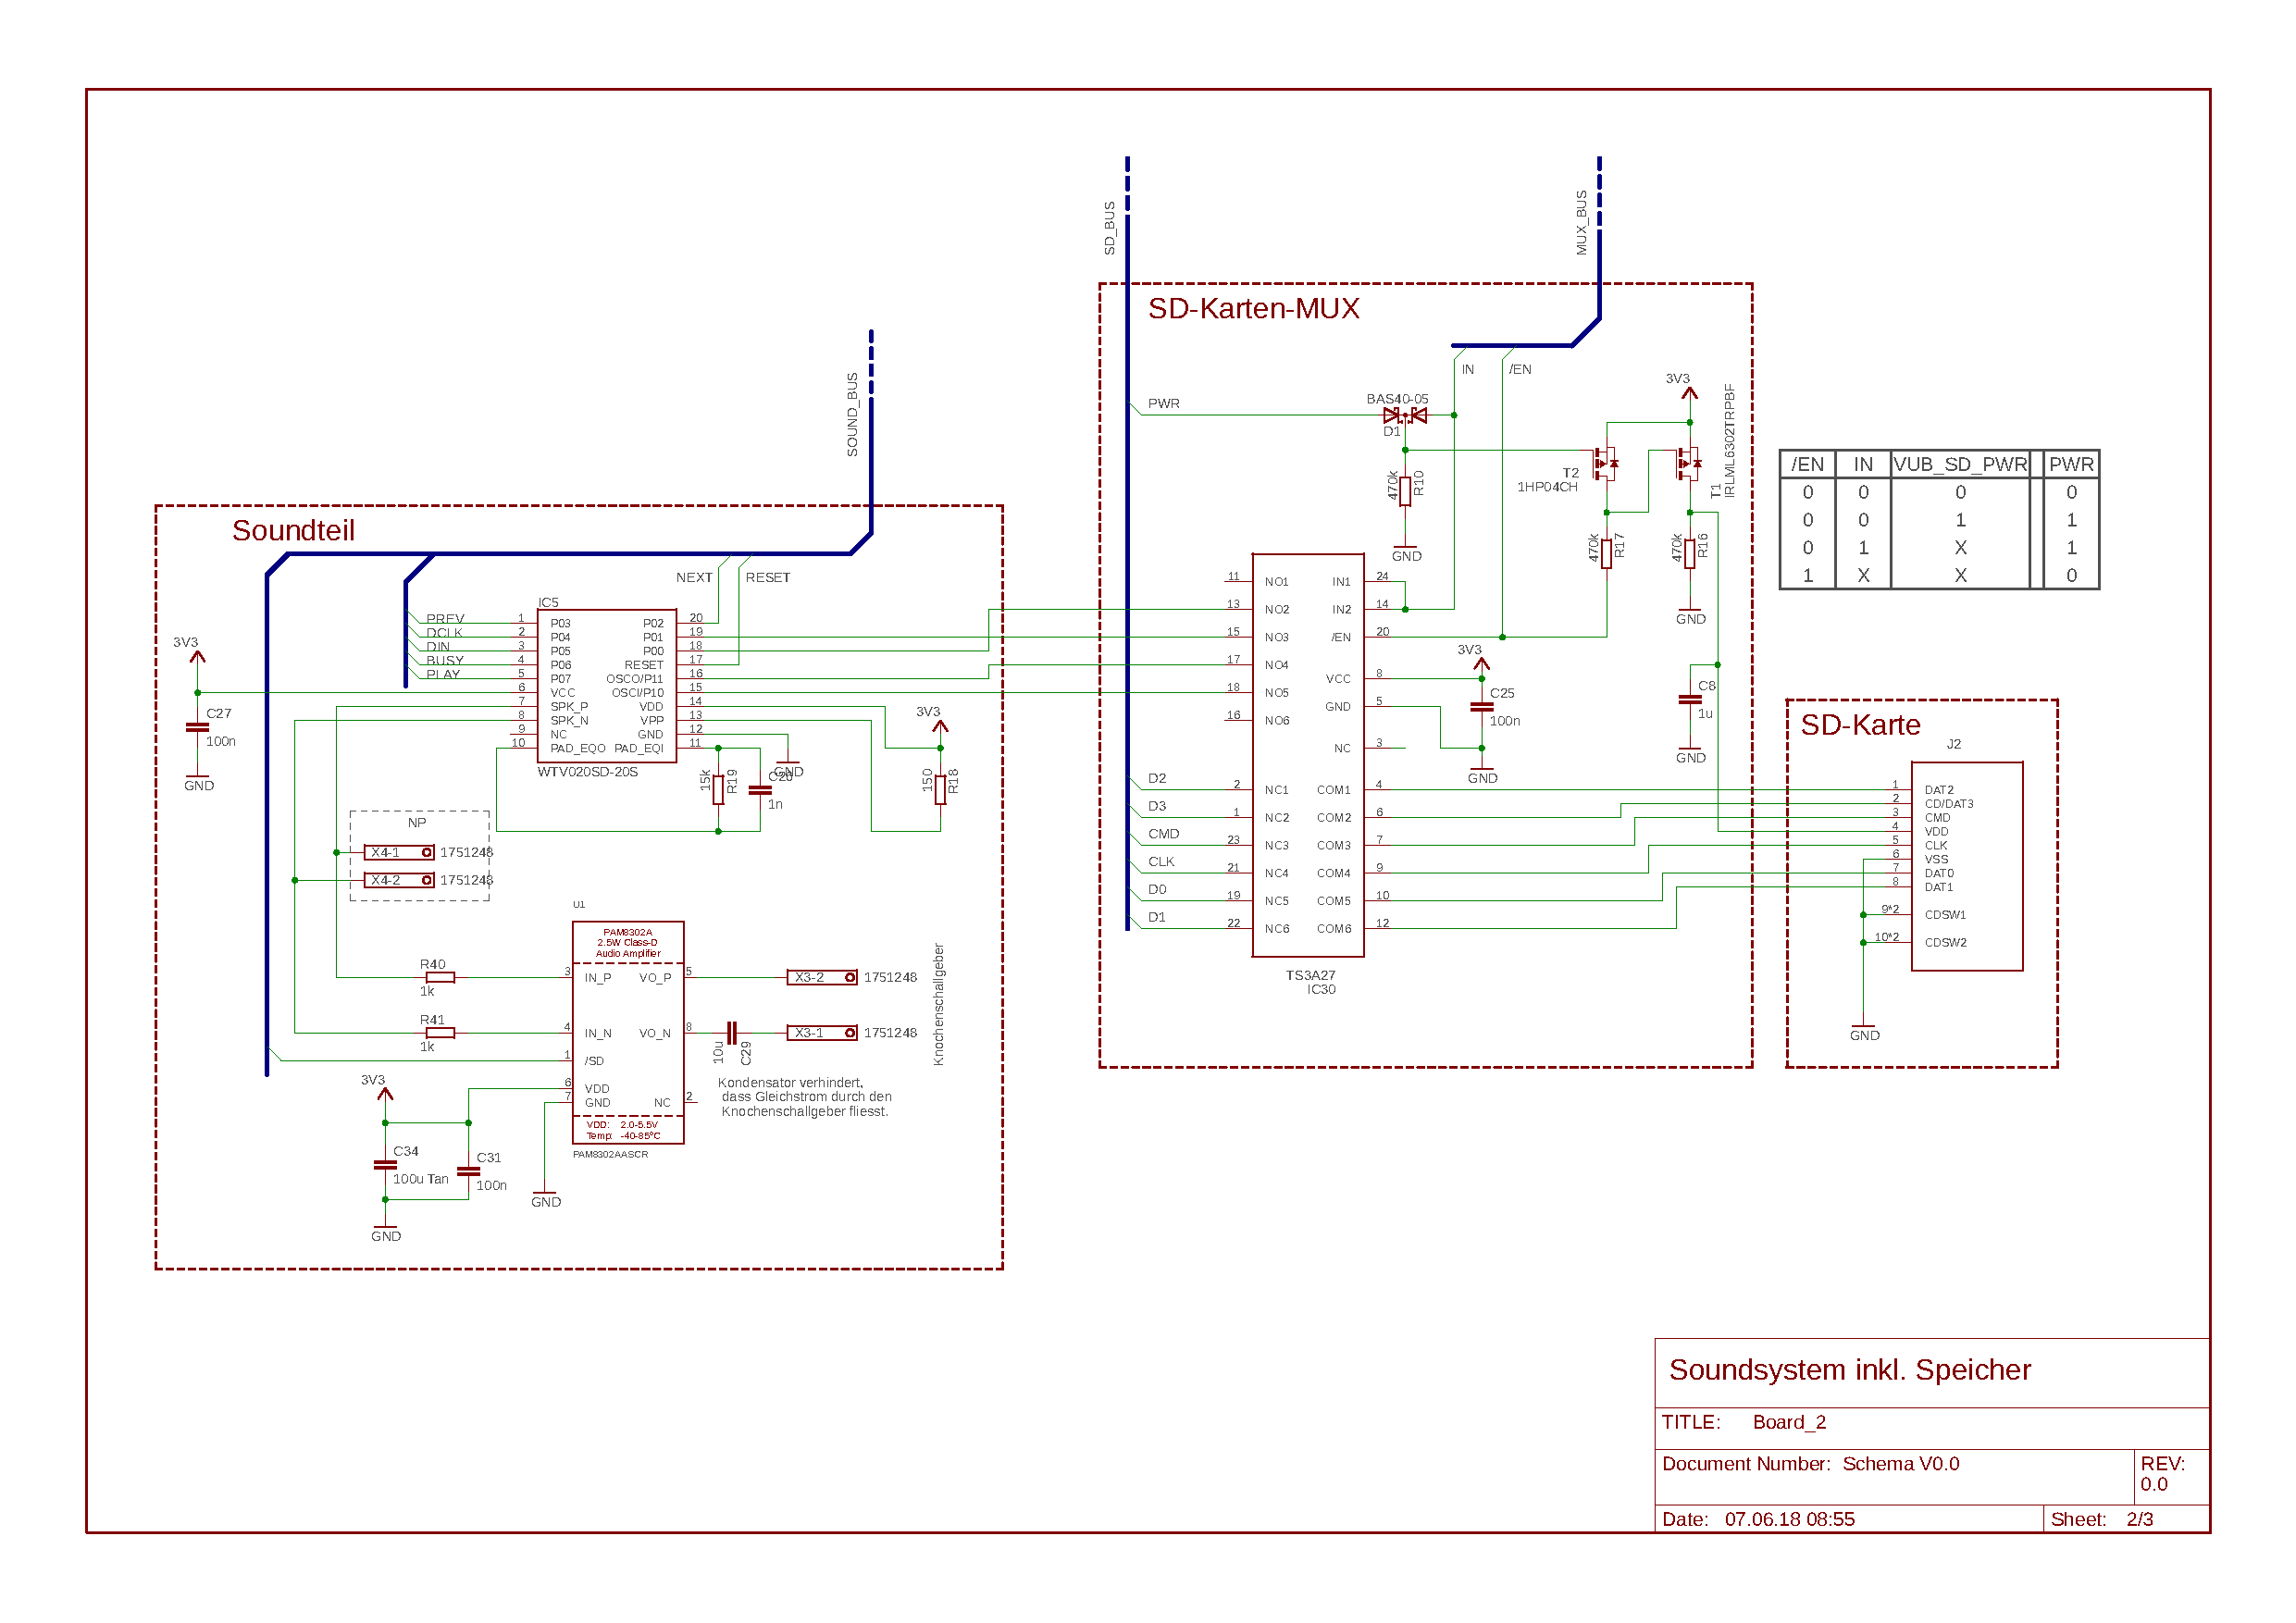
\includepdf[fitpaper]{Board_22.pdf}

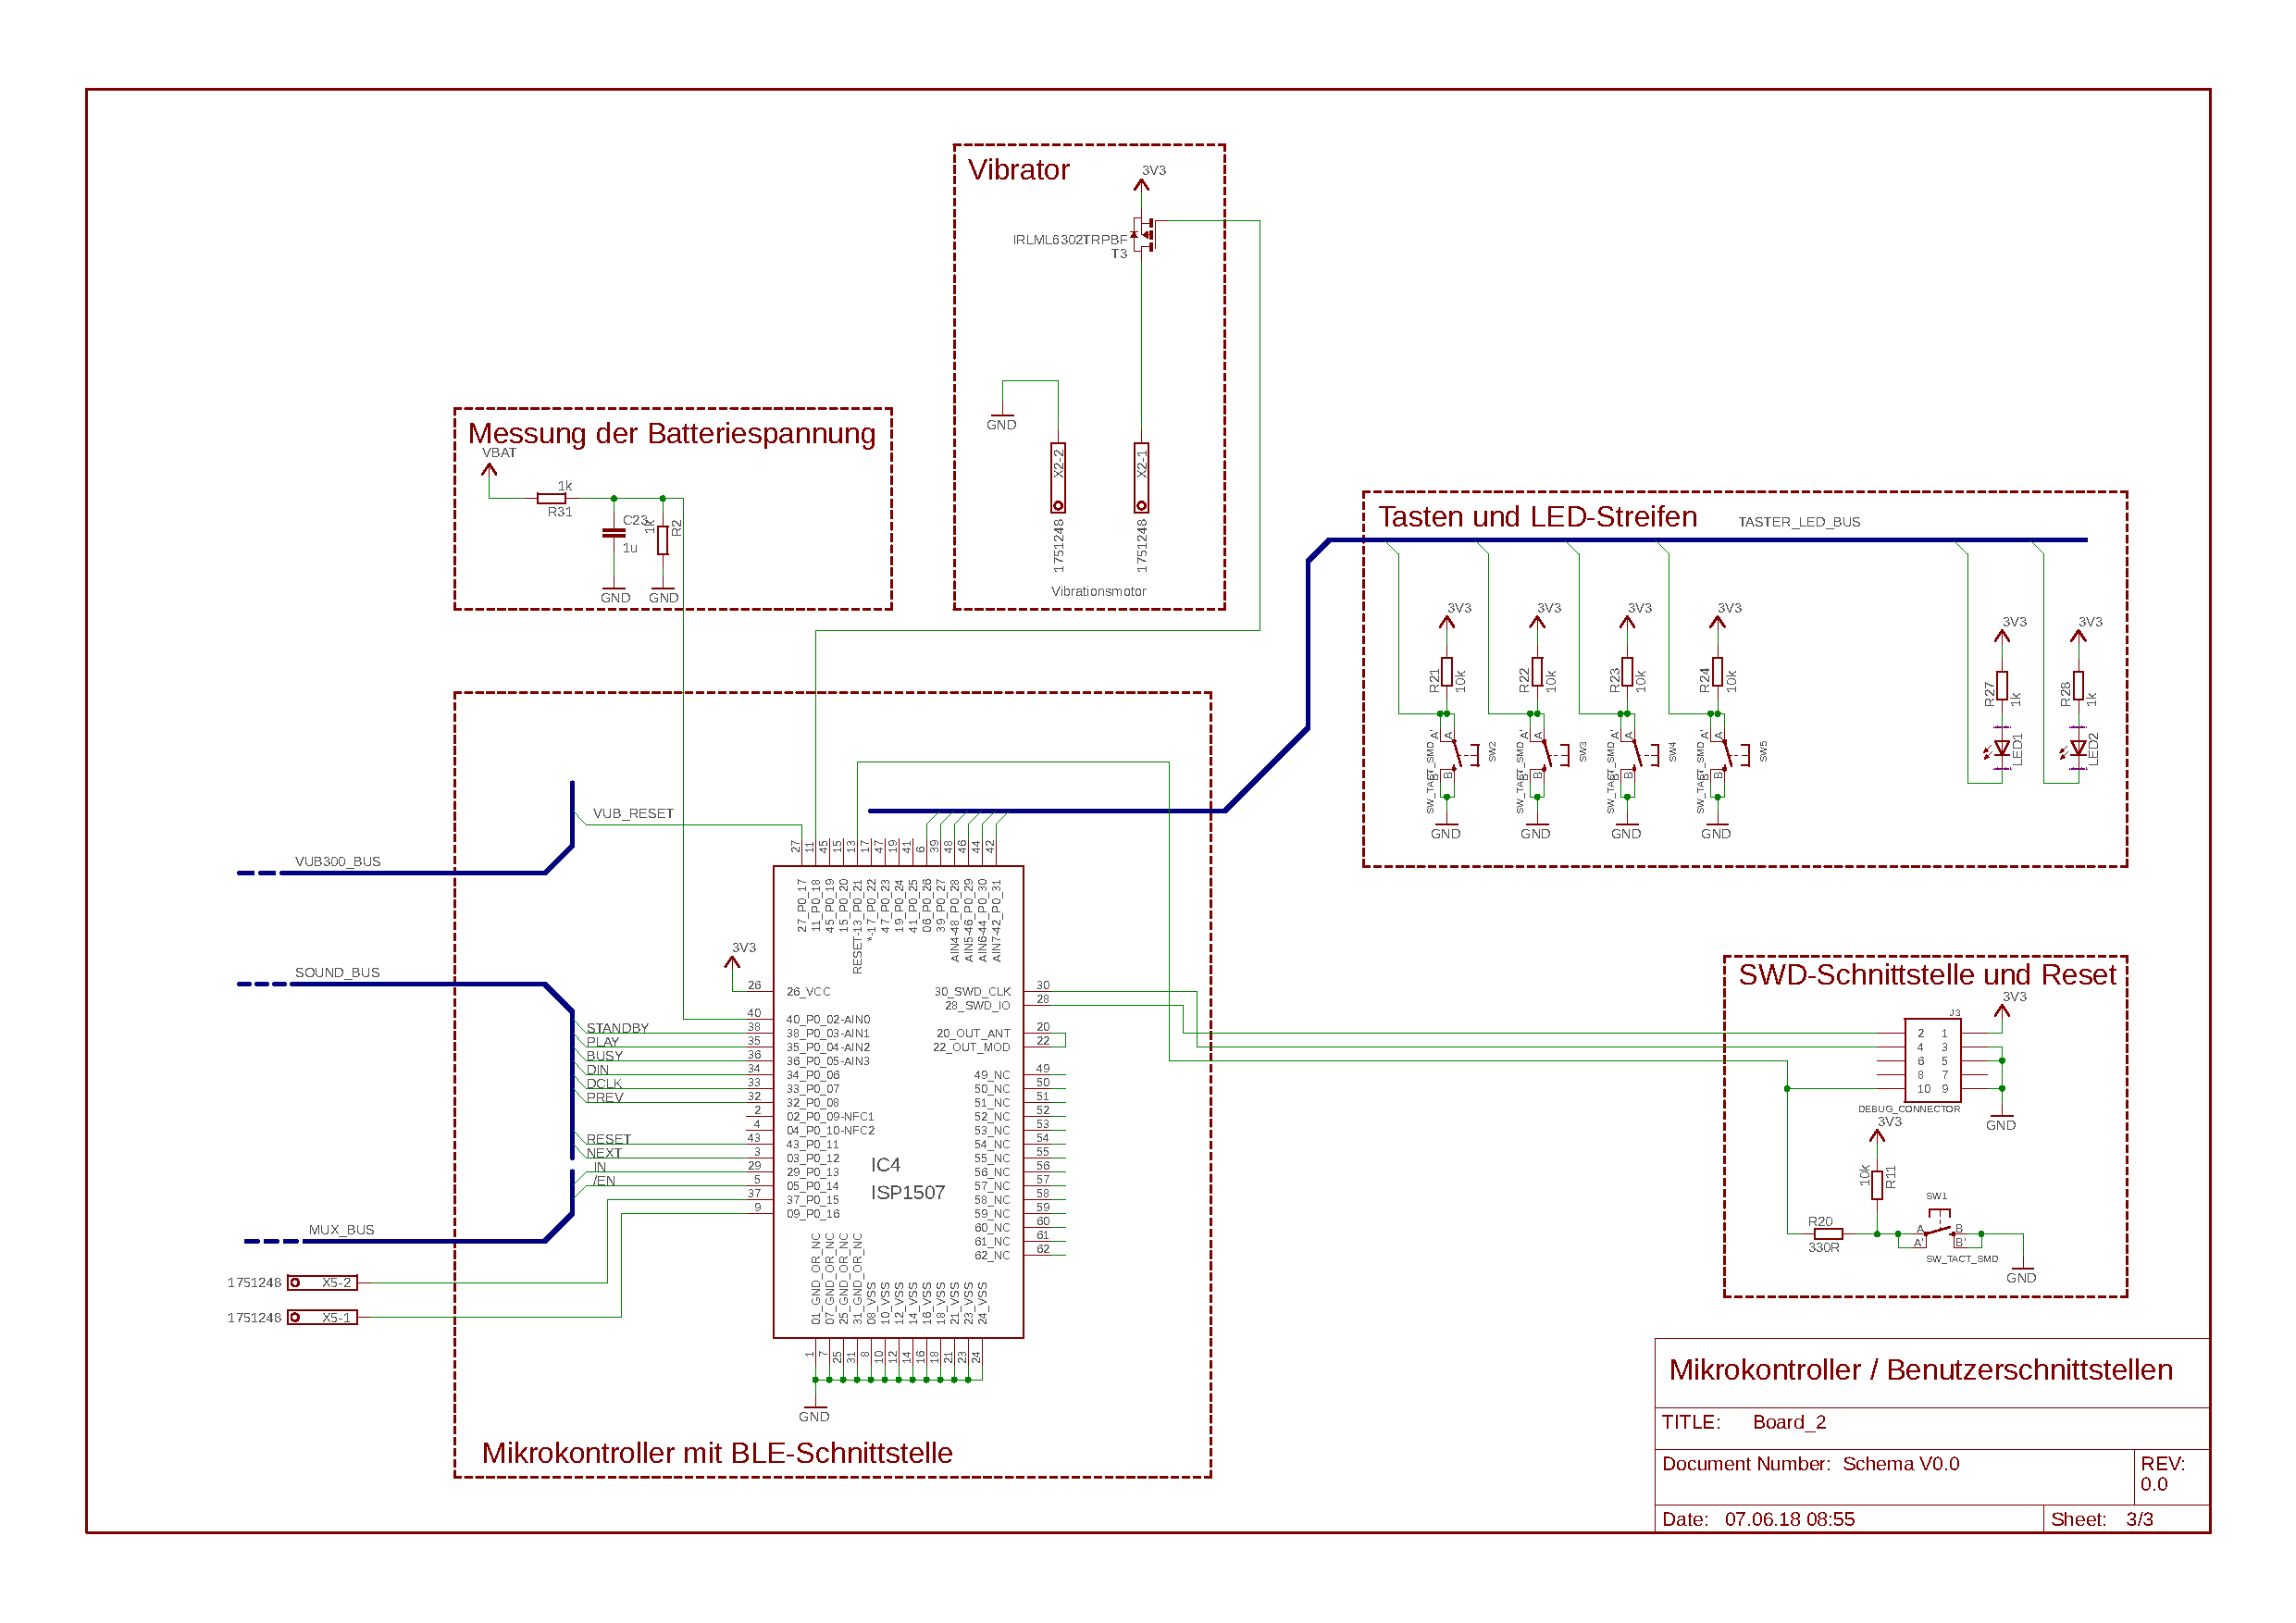
\includepdf[fitpaper]{Board_23.pdf}

\section{Softwarekonzept}

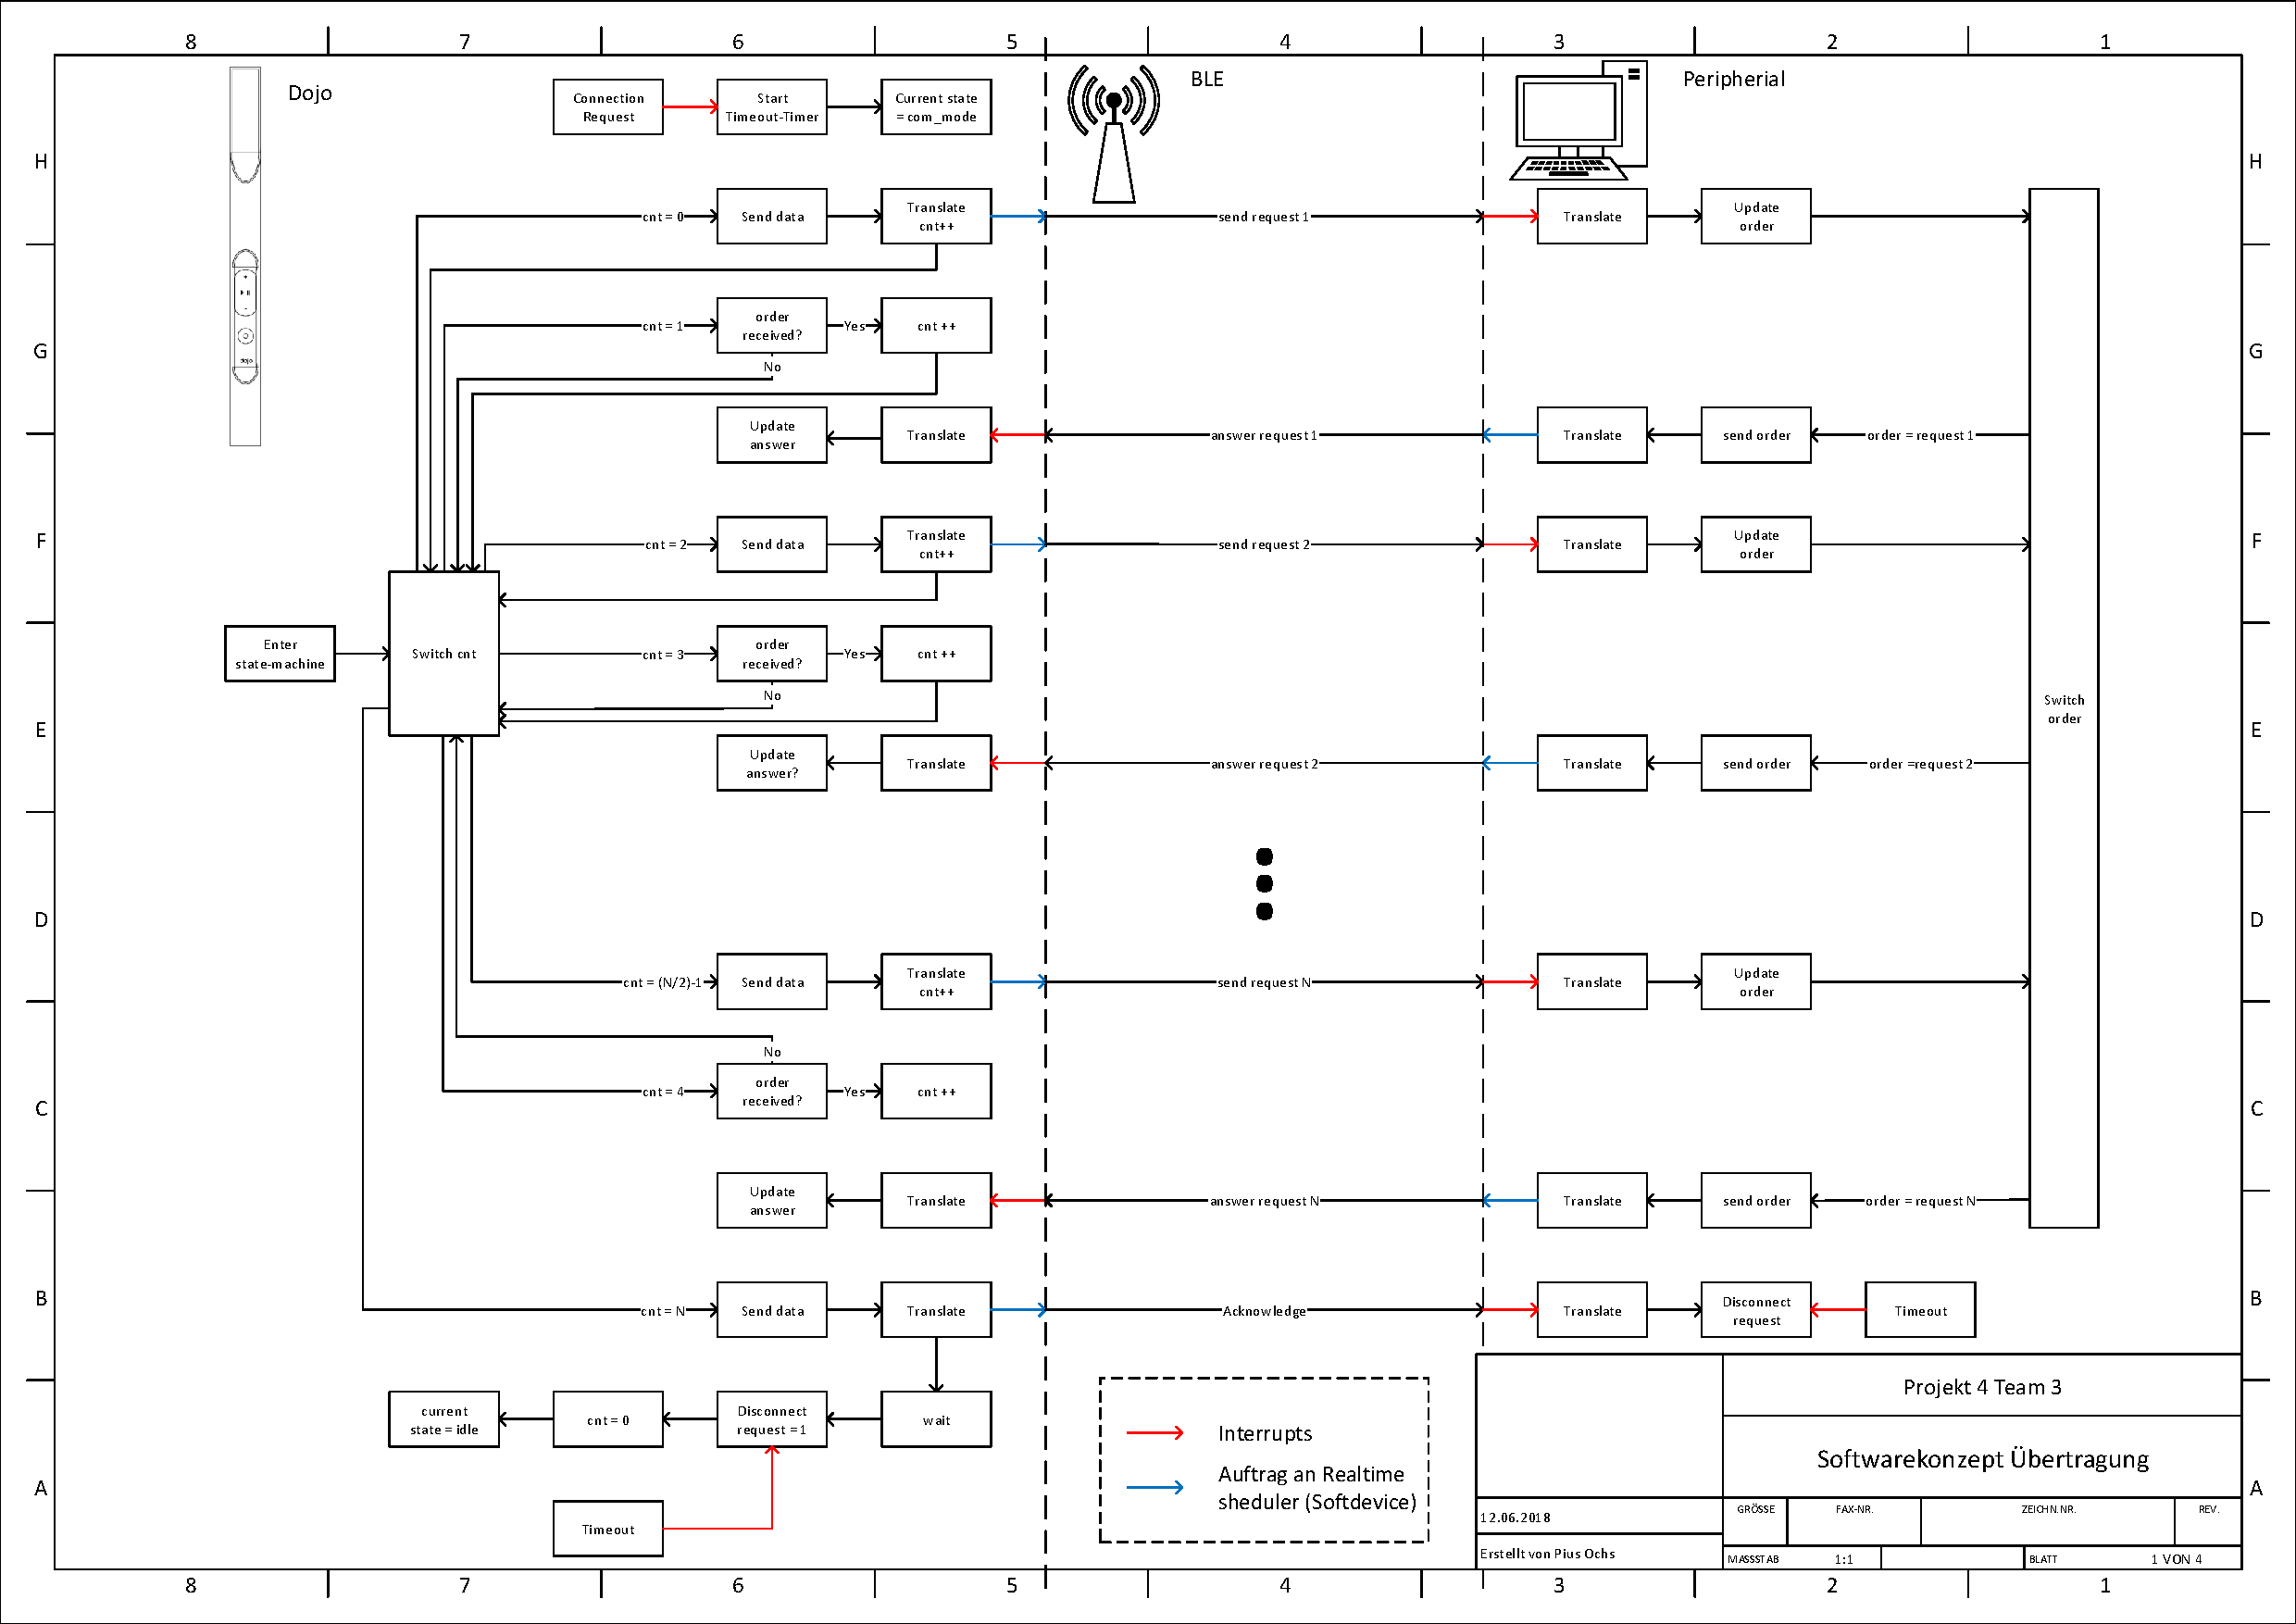
\includepdf[fitpaper]{Softwarekonzeptzeichnung1.pdf}
\label{Softwarekonzeptzeichnung1.pdf}

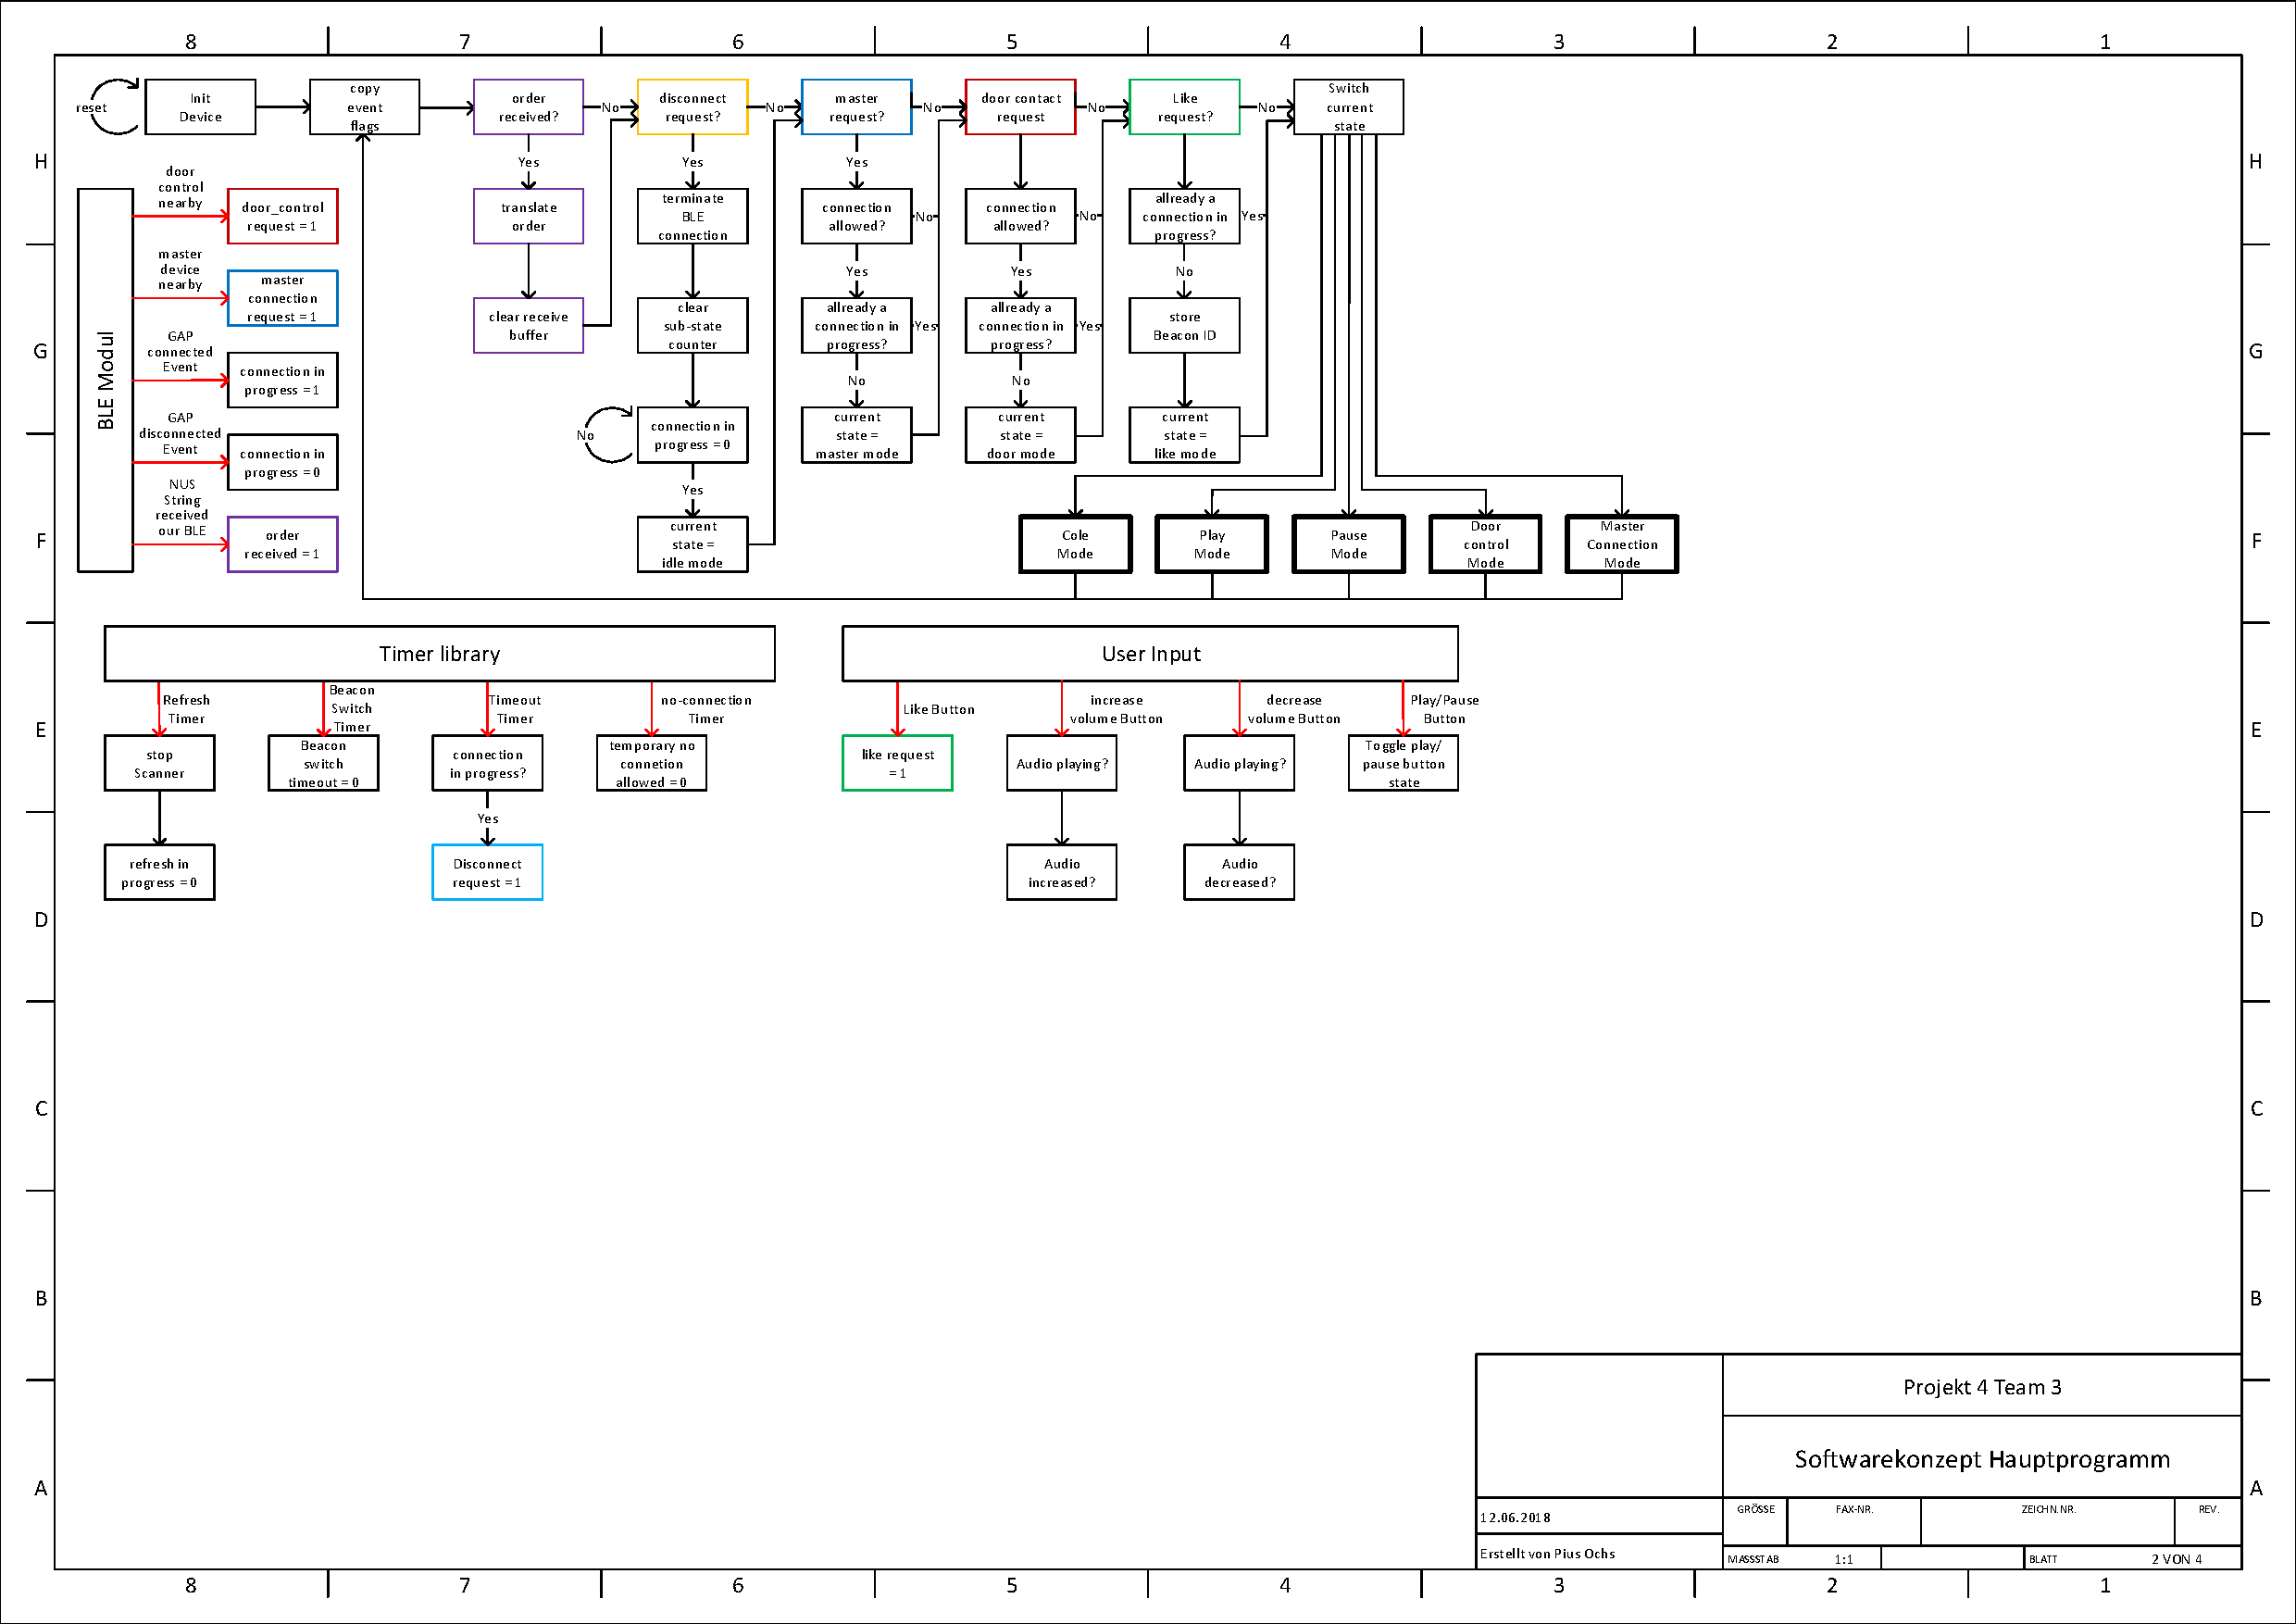
\includepdf[fitpaper]{Softwarekonzeptzeichnung2.pdf}
\label{Softwarekonzeptzeichnung2.pdf}

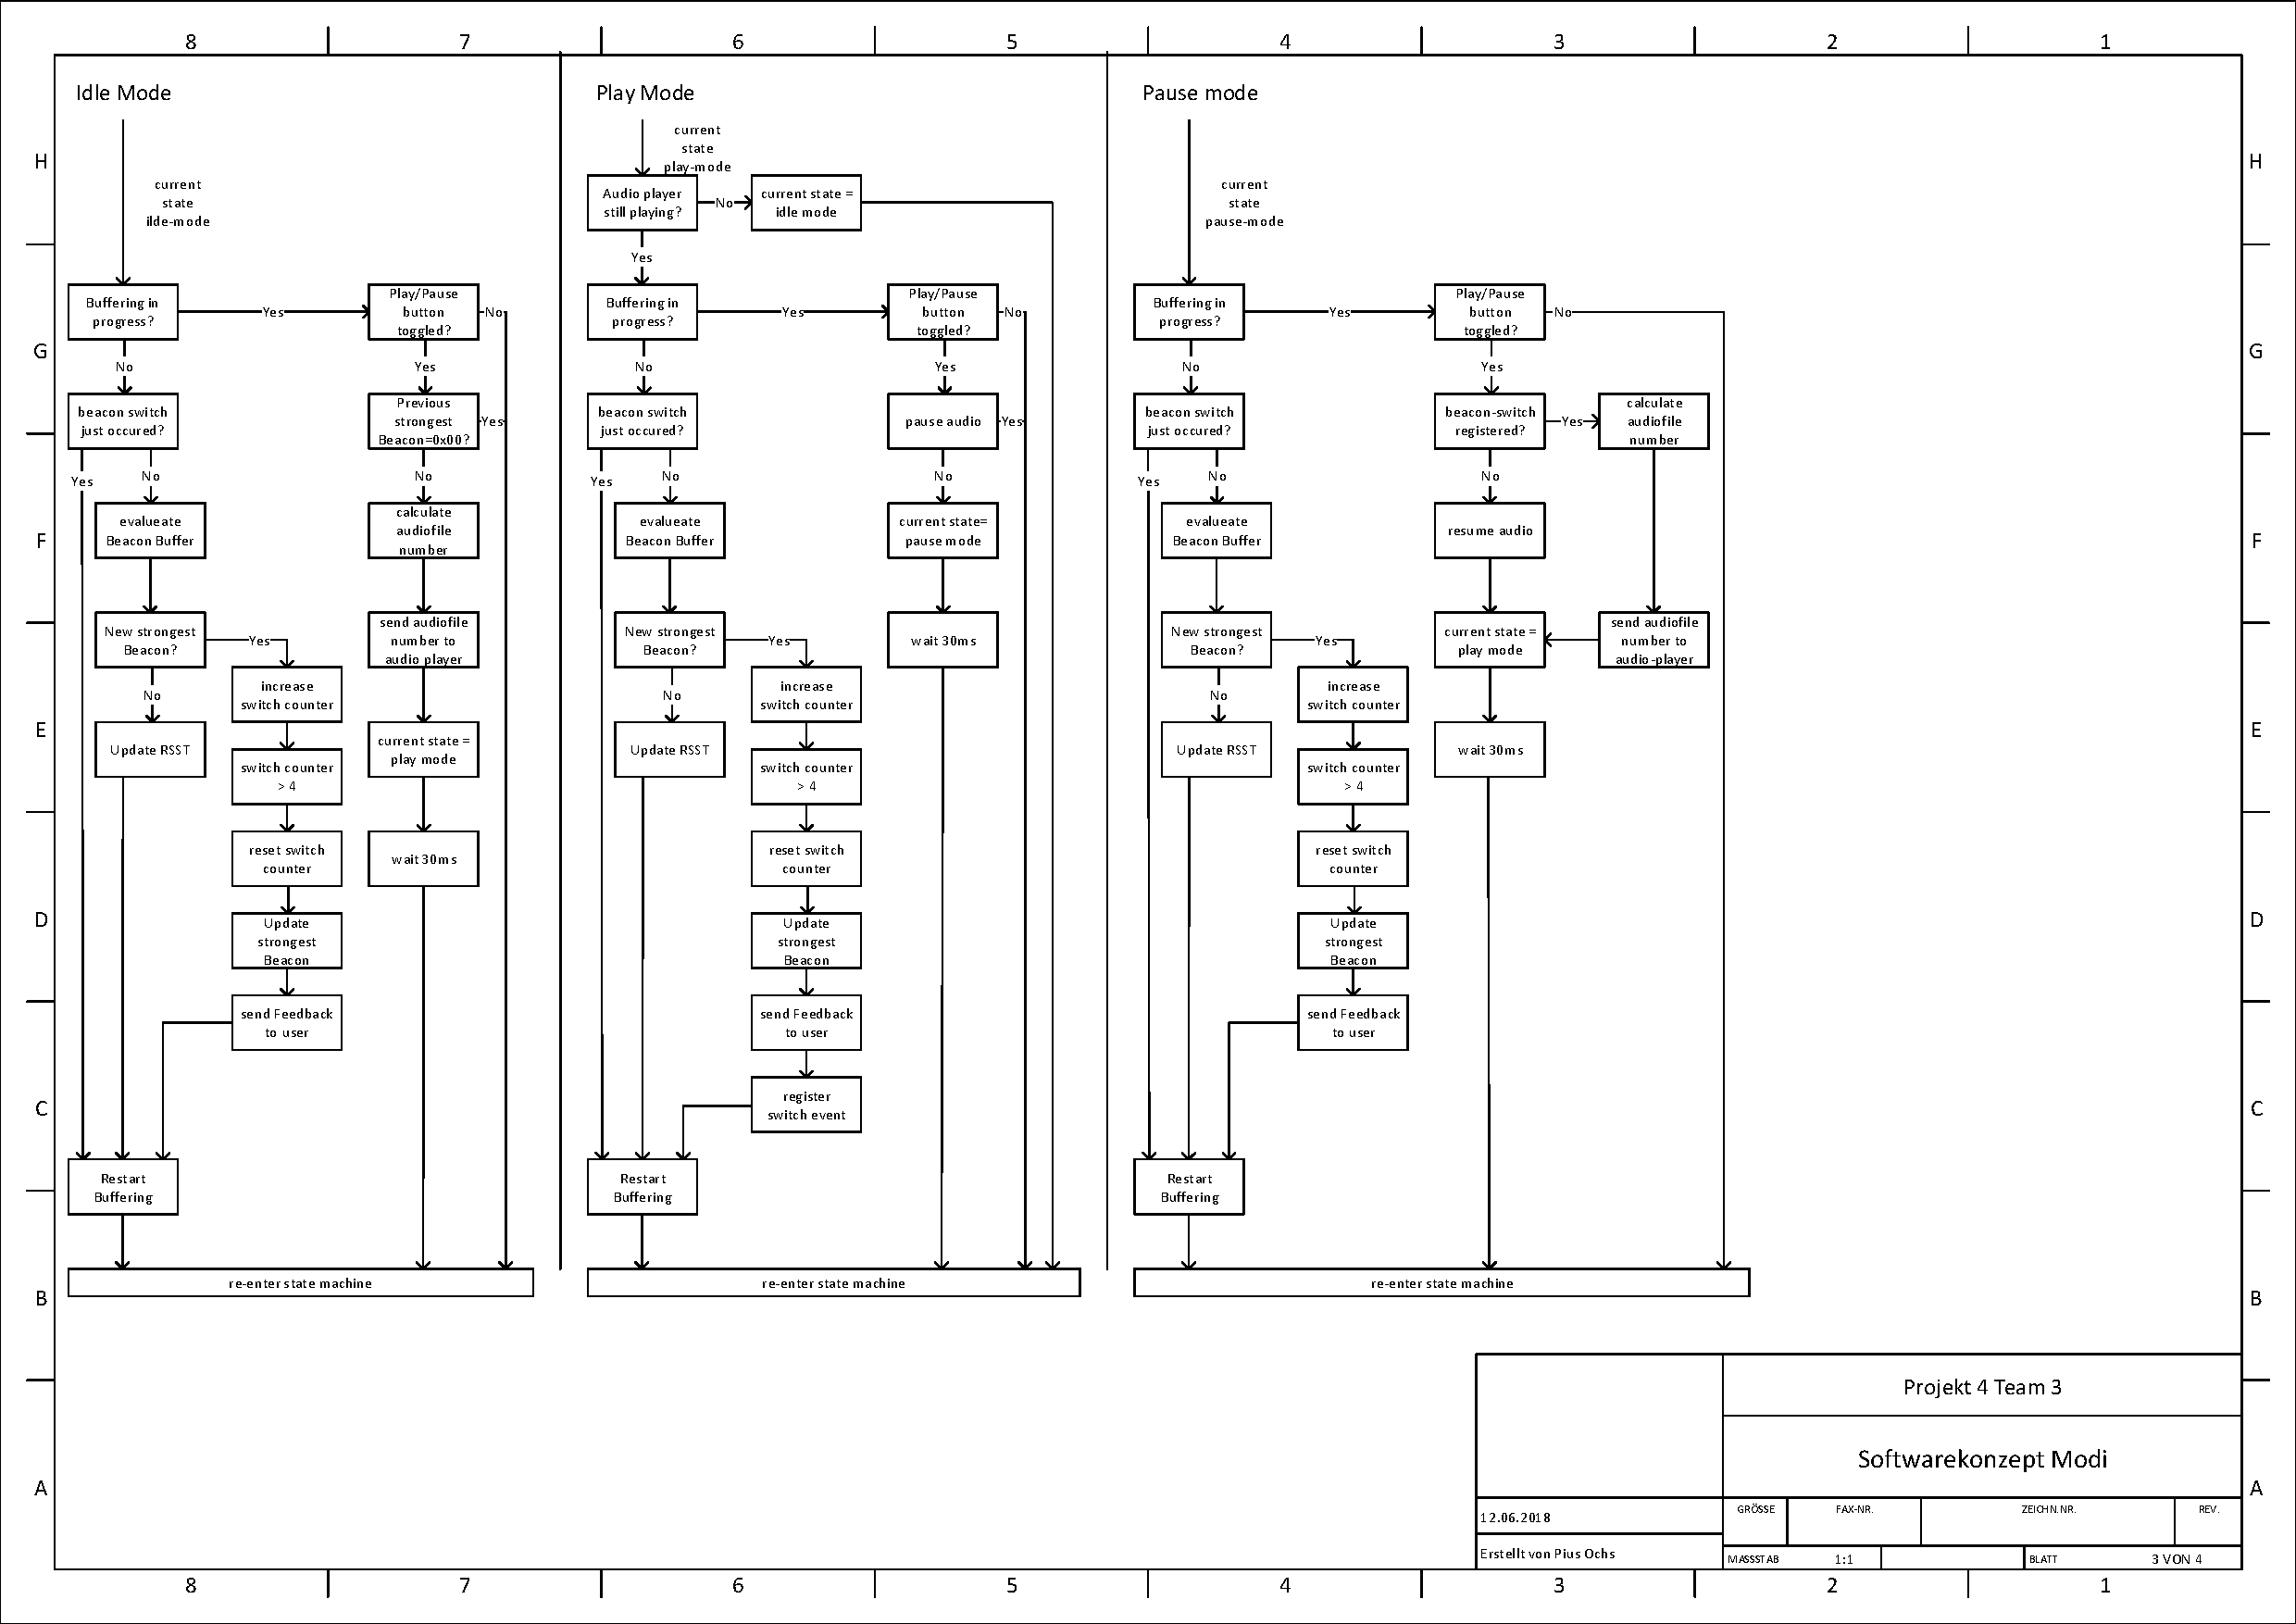
\includepdf[fitpaper]{Softwarekonzeptzeichnung3.pdf}
\label{Softwarekonzeptzeichnung3.pdf}

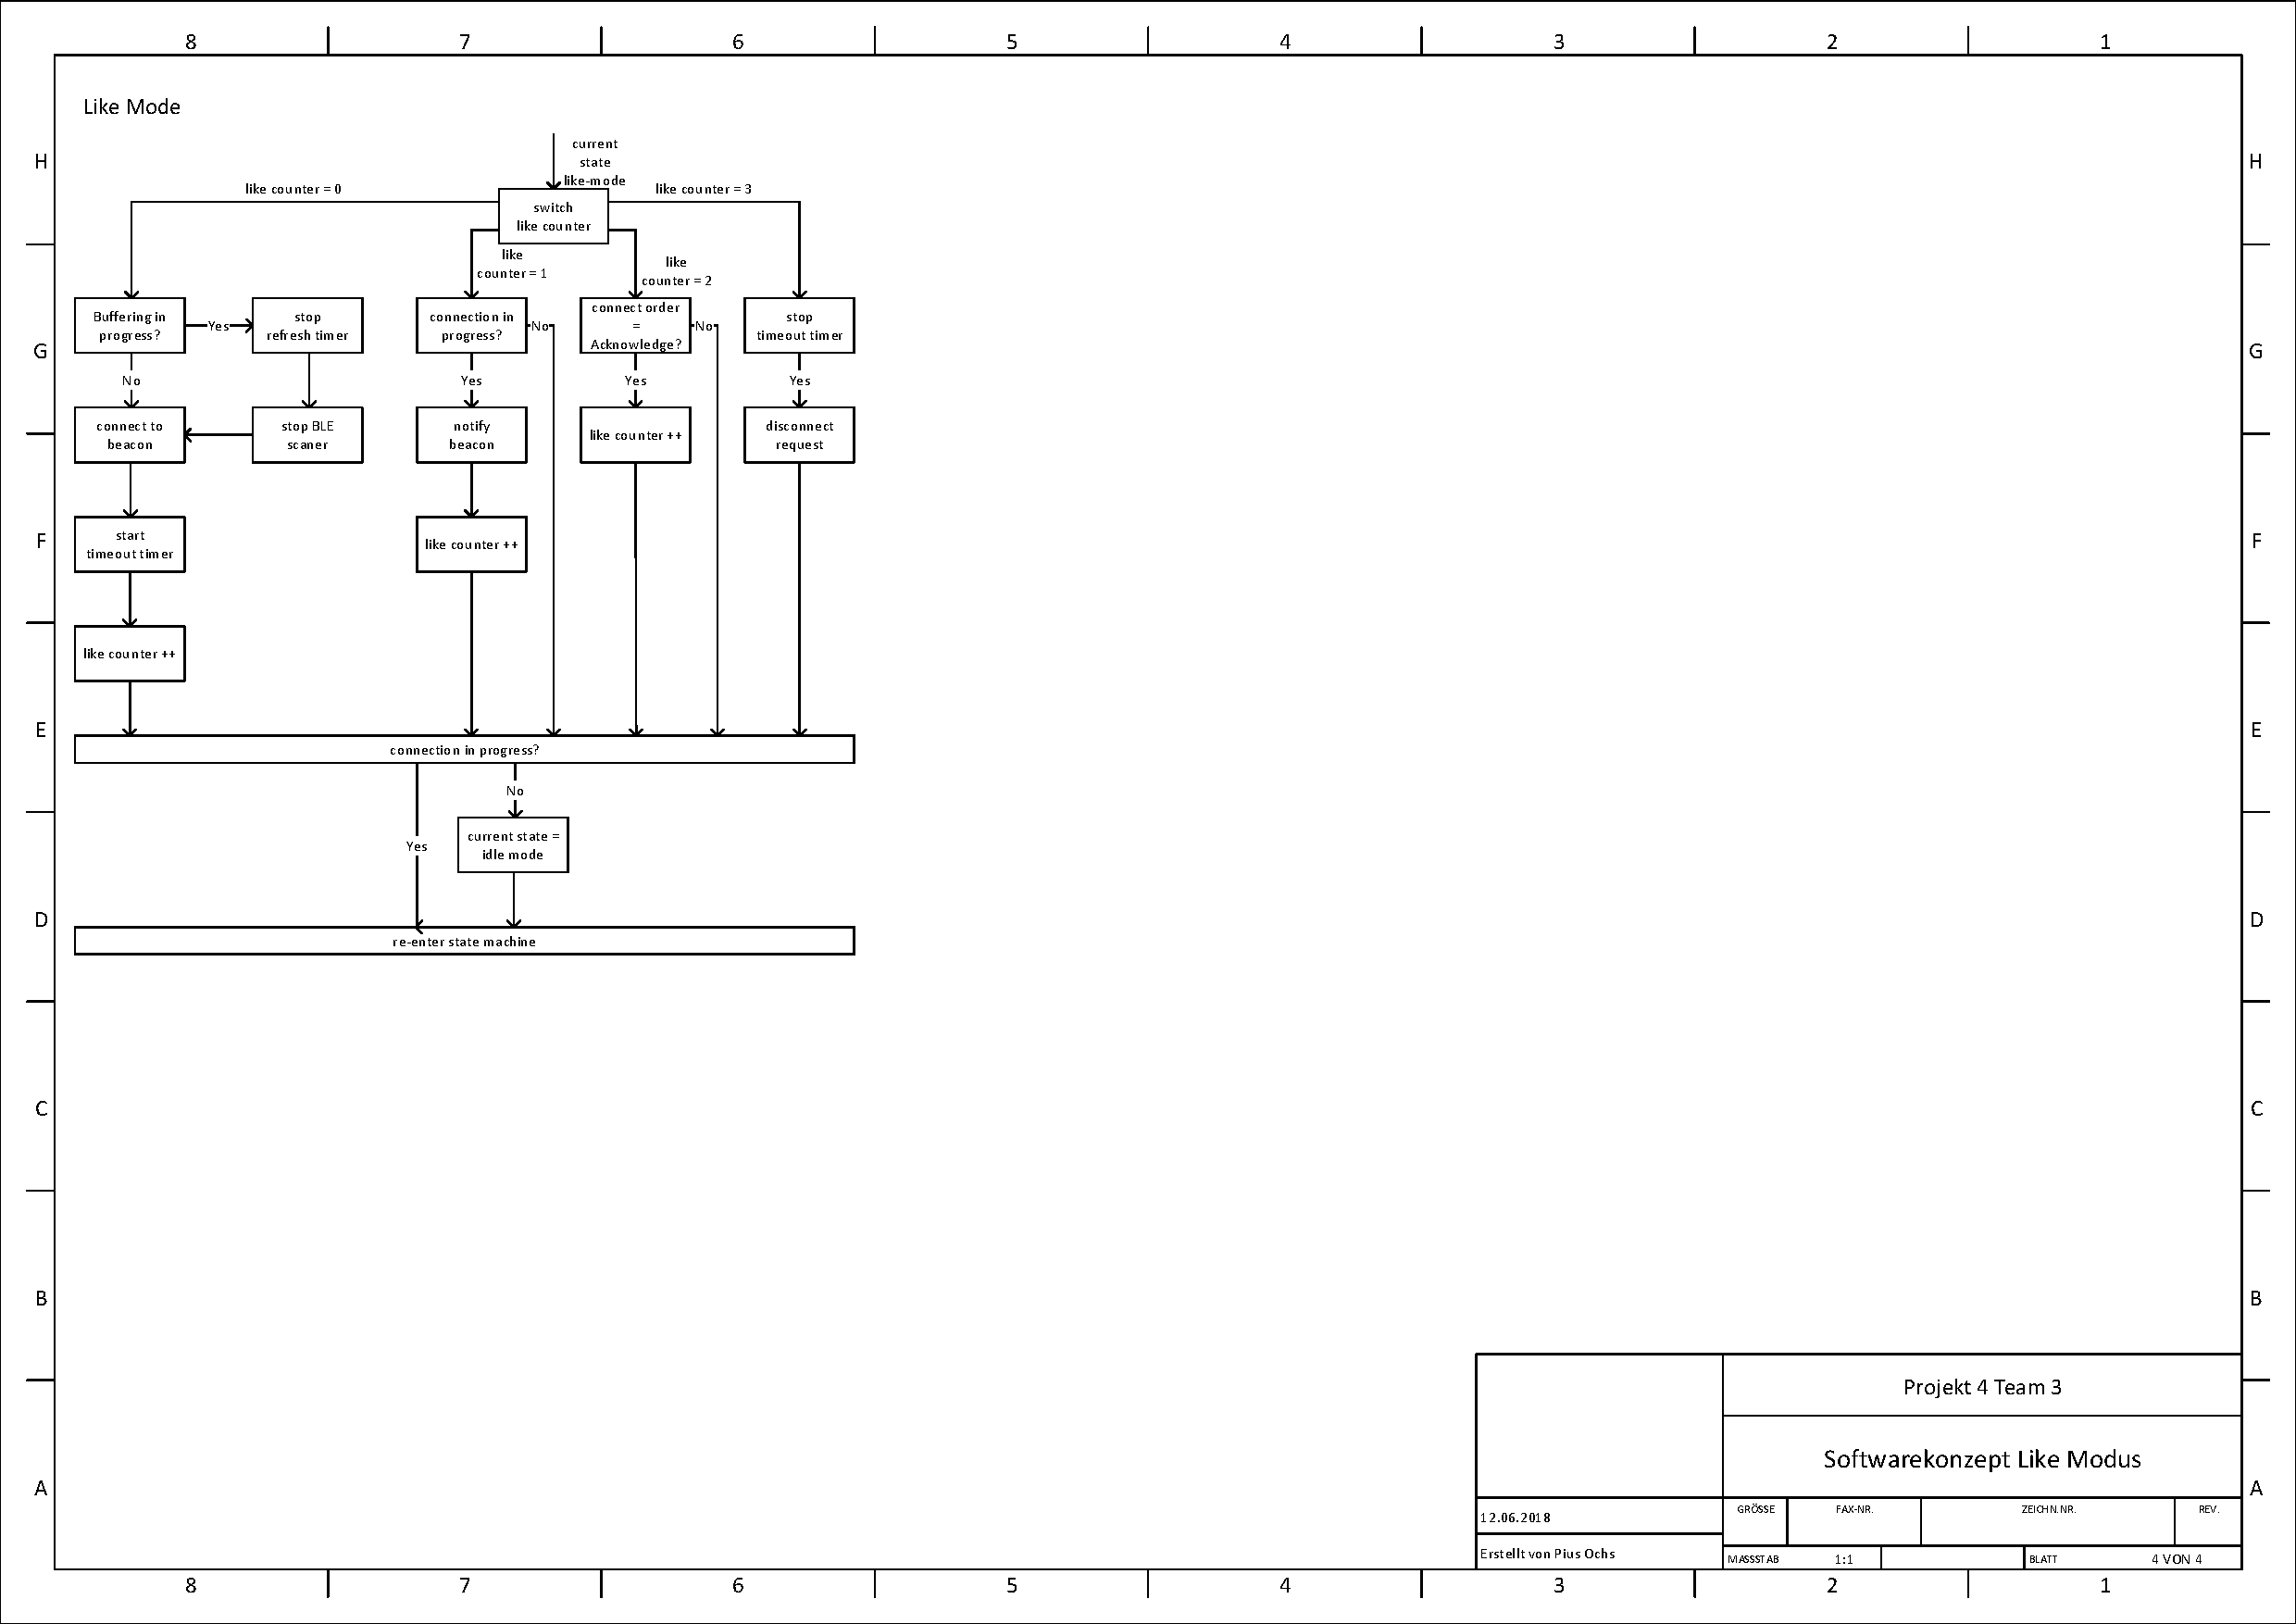
\includepdf[fitpaper]{Softwarekonzeptzeichnung4.pdf}
\label{Softwarekonzeptzeichnung4.pdf}